\documentclass[12pt]{ociamthesis}  % default square logo 
%\documentclass[12pt,beltcrest]{ociamthesis} % use old belt crest logo
%\documentclass[12pt,shieldcrest]{ociamthesis} % use older shield crest logo

%load any additional packages
\usepackage{titlesec} %section font
\usepackage{amssymb}
\usepackage{multirow}
\usepackage{hyperref}
\usepackage{float}
\usepackage[normalem]{ulem}
\renewcommand{\labelenumii}{\theenumii}               %buat enumerate
\renewcommand{\theenumii}{\theenumi.\arabic{enumii}.} %
\useunder{\uline}{\ul}{}
\usepackage{caption}
%%%%%%%% untuk enum 1.1 dan a
\usepackage{amsmath}  %for '\tag' macro and 'align' env
\usepackage{amsfonts}
\usepackage{verbatim}
\usepackage{array}
\usepackage{textcomp}
\usepackage{enumitem}
%%%%%%%%
\usepackage{tabularx}
\usepackage{graphicx}
\usepackage{adjustbox}

%%%%%%%%%
\titleformat{\chapter}[block]{\bfseries\centering\fontsize{16pt}{16pt}\selectfont}{\chaptertitlename~\thechapter.}{12pt}{}
\titleformat{\section}
  {\normalfont\fontsize{14}{15}\bfseries}{\thesection}{1em}{}
%input macros (i.e. write your own macros file called mymacros.tex 
%and uncomment the next line)
%\include{mymacros}

\title{ PEDOMAN	PROYEK	II \\
DEBUGGER TANGGUH \\
D4	TEKNIK	INFORMATIKA}   %note \\[1ex] is a line break in the title

\author{}             %your name
\college{}  %your college

%\renewcommand{\submittedtext}{change the default text here if needed}
\degree{Politeknik Pos Indonesia}     %the degree
\degreedate{Bandung}         %the degree date
\degreedate{2019}  

%end the preamble and start the document
\begin{document}

%this baselineskip gives sufficient line spacing for an examiner to easily
%markup the thesis with comments
\baselineskip=18pt plus1pt

%set the number of sectioning levels that get number and appear in the contents
\setcounter{secnumdepth}{3}
\setcounter{tocdepth}{3}


\maketitle                  % create a title page from the preamble info
\begin{dedication}

”Barang siapa yang menghendaki kehidupan dunia maka wajib baginya memiliki ilmu, \\
dan barang siapa yang menghendaki kehidupan Akherat, \\ 
maka wajib baginya memiliki ilmu, \\
dan barang siapa menghendaki keduanya maka wajib baginya memiliki ilmu”. \\
(HR. Turmudzi) \\

\end{dedication}        % include a dedication.tex file
\begin{acknowledgements}
Pertama-tama	 kami	 panjatkan	 puji	 dan	 syukur	 kepada	Allah	SWT	 yang	 telah	memberikan	rahmat	 dan	 hidayah-Nya	 sehingga	 Buku	 Pedoman	 dan	 Kegiatan	 Proyek	Debugger Tangguh (PROYEK	II)	ini	dapat	diselesaikan.

Buku	 Pedoman	 ini	 dibuat	 dengan	 tujuan	 memberikan	 acuan,	 baik	 bagi	 mahasiswa	 yang	
akan	mengambil	matakuliah	Proyek	Debugger Tangguh	(PROYEK	II)	maupun	bagi	dosen	pembimbing.	Pada	intinya	buku	ini	menjelaskan	secara	lengkap	tentang	Karakteristik	PROYEK	II	
di	 Program	 Studi	 Teknik	 Informatika,	 dan	 juga	 mengatur	 mekanisme,	 teknik	 penulisan,	 serta	
penilaiannya.Dengan	demikian	diharapkan	semua	pihak	yang	terlibat	dalam	aktivitas	PROYEK	II	
mempunyai	kesamaan	dalam	pelaksanaannya

Tak	 ada	 gading	 yang	 tak	 retak,	 tak	 ada	 manusia	 yang	 sempurna	 dan	 apapun	 yang	
dihasilkannya,	sehingga	koreksi	serta	masukan	untuk	berbagai	kekurangan	dalam	Buku	Pedoman	
dan	 Kegiatan	 Pemrograman	 dan	 Jaringan	 (PROYEK	 II)	 ini	 tetap	 diharapkan.	 Terimakasih	 atas	
kerjasama	 banyak	 pihak,	 dan	 semoga	 buku	 ini	 memberikan	 banyak	 manfaat	 khususnya	 bagi	
pihak-pihak	yang	terkait.


\begin{raggedright}

Bandung,  September 2019 \\
Ketua	Prodi	DIV	Teknik	Informatika\\[8ex]


\underline{M.	Yusril	Helmi	Setyawan,	S.Kom.,	M.Kom.}\\
NIK.113.74.163

\end{raggedright}

\end{acknowledgements}   % include an acknowledgements.tex file

\begin{romanpages}          % start roman page numbering
\tableofcontents            % generate and include a table of contents
\end{romanpages}            % end roman page numbering

%now include the files of latex for each of the chapters etc
\chapter{PERATURAN UMUM}
\section{Pendahuluan}
Pendidikan profesional bertujuan untuk menghasilkan tenaga kerja yang siap pakai. Lulusan yang siap pakai adalah ciri yang membedakan antara pendidikan profesional dengan pendidikan akademis. Selama masa pendidikan, mahasiswa Politeknik Pos Indonesia dipersiapkan dan dilatih agar kelak mempunyai kemampuan untuk beradaptasi secepatnya dengan dunia kerja.

Untuk melatih mahasiswa Politeknik Pos Indonesia dalam hal implementasi serta mewujudkan hasil implementasinya, mahasiswa diwajibkan mengerjakan  Proyek	Debugger Tangguh. Dengan tugas tersebut diharapkan mahasiswa dapat menerapkan ilmu dan pengetahuan yang telah dipelajari sebelumnya. Diharapkan pula, mahasiswa mampu mengidentifikasi persoalan, implementasi, menentukan spesifikasi,serta mampu mengukur dan mencari kesalahan (\textit{trouble shooting}) hasil yang di implementasikannya.

\section{Nama Kegiatan}
\textbf{Proyek	Debugger Tangguh }

\section{Tujuan}
Proyek	Debugger Tangguh termasuk mata kuliah yang harus ditempuh sebagaimana mata-mata kuliah lainnya pada program pendidikan Diploma IV Politeknik Pos Indonesia yang bertujuan memberikan kesempatan kepada mahasiswa untuk mengimplementasikan pengetahuan teori dan praktek yang didapat dalam bentuk suatu pekerjaan proyek.\textit{ Dengan menambahkan fitur web service dan network security}.\textbf{Web service wajib menggunakan Oauth atau sistem Token buatan sendiri}. Database menggunakan fungsi dan atau prosedur dan atau trigger. Penggunaan atau implementasi database cache pada aplikasi proyek 2 menggunakan \textbf{redis} akan menjadi nilai lebih.

\section{Waktu}
Proyek	Debugger Tangguh  dikerjakan pada semester 3.

\section{Tahap-Tahap Pelaksanaan Proyek}
Dalam melakukan pelaksanaan	proyek harus berdasarkan tahapan-tahapan	yang dijelaskan	sebagai	berikut	:
\begin{enumerate}
\item Pemilihan topik dari proyek yang akan dikerjakan ;

\item Pengajuan proposal proyek ke dosen calon pembimbing yang telah ditentukan sebelumnya oleh koordinator proyek ;

\item Proses review oleh dosen calon pembimbing	untuk disetujui, kemudian proposal dikumpulkan ke	prodi untuk	mendapatkan	form nilai	bimbingan proyek II ;

\item Proses bimbingan yang	berkaitan dengan pembuatan aplikasi	dan penyusunan laporan yang diarahkan oleh dosen pembimbing masing-masing	untuk diberikan pengesahan penilaian proses	bimbingan perminggu.

\item Pelaksanaan sidang untuk menguji dan menilai hasil akhir dari	 kegiatan proyek yang dilakukan sebelumnya.
\end{enumerate}

\section{Proses Pemilihan Topik Proyek}
Topik Proyek dapat berasal dari	mahasiswa atau pembimbing proyek II.	 Prosedur pemilihan topik untuk keduanya	adalah sebagai berikut :


\begin{figure}[H]
    \centering
    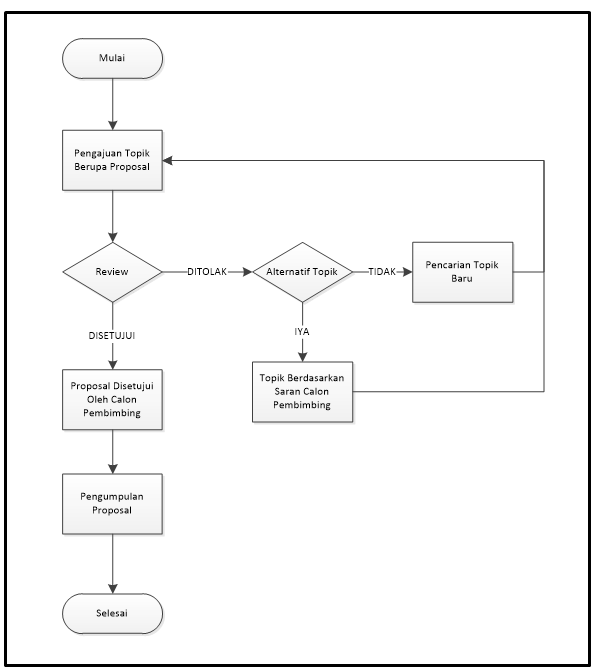
\includegraphics[scale=0.7]{figures/alur.png}
    \caption{Diagram Alir Pemilihan dan Pengajuan Topik}
    \label{alir}
\end{figure}

\section{Pengajuan Topik dan Penetapan Pembimbing Proyek}
Topik diajukan ke Koordinator Proyek dengan	menggunakan	proposal dalam	bentuk \textbf{luring dan daring}. Berdasarkan hasil penilaian \textit{reviewer}, maka Koordinator Proyek menerima atau menolak proposal yang diajukan dan menetapkan pembimbing (Lihat \textit{Flowchart} Proses Pengajuan hingga Sidang Proyek).

\section{Peraturan Pelaksanaan Proyek II}
Dalam pelaksanaan Proyek II	ini	ada	beberapa aturan	yang ditentukan	diantaranya	sebagai	berikut	:

\begin{enumerate}
	\item Telah	 Mengikuti	 dan	 lulus	 pada	 Kegiatan	 Character	 Building	 di	 Politeknik	 Pos Indonesia yang	dikuatkan	dengan	melampirkan	Fotocopy	Sertifikat.
	
	\item Telah	Mengikuti	 dan	lulus	 pada	 Kegiatan	MORRIS	 Program	 Studi	 Teknik	 Informatika yang dikuatkan	dengan	melampirkan	Fotocopy	Sertifikat.
	
	\item Lulus	minimal	C	untuk	4	mata	kuliah	Web	Service,	Basdat,	RPL, Jarkom, Mobile, Metlid, Admin	Jarkom.
	
	\item Pada	 saat	 pengumpulan	 proposal	 disertakan	 KRS	 dan	 DHS, yang langsung dikumpulkan	di	admin.
	
	\item Satu kelompok terdiri atas maksimal 2 orang dan memiliki 1 tema.
	
	\item Jika terlambat mengumpulkan Proposal (tidak sesuai dengan	jadwal yang telah	ditentukan) maka	 akan	 dinyatakan	\textbf{TIDAK LULUS} dan	 tidak	 diperkenankan	 mengajukan	 judul kembali.	\textit{\textbf{(dianggap mengulang proyek pada semester berikutnya)}} ;
	
	\item Jika Proposal	yang ditolak maka diberikan waktu 1 minggu untuk pengajuan ulang	Proposal	Proyek	II,	jika penolakan	melebihi 3	kali maka dinyatakan	\textbf{TIDAK LULUS} dan tidak	 diperkenankan	 mengajukan judul kembali. \textit{\textbf{(dianggap mengulang proyek pada semester berikutnya)}} ;
	
	\item Penilaian	Proses	Bimbingan	:	Diberikan	total	waktu selama 10 minggu, setiap minggu	mendapat 1 penilaian proses	bimbingan dengan	nilai sebesar maksimal 10 terdiri dari penilaian \textit{ uniqeness} 300	 kata tulisan blog (50\%), 10 \textit{commit} standard github (25\%), dan video log standard (25\%) yang berisi tentang pengerjaan pada waktu minggu tersebut, keterlambatan pengerjaan tidak akan mendapatkan toleransi ( Nilai 0 ). Sehingga nilai total untuk 10 minggu jumlahnya 100. Jika nilai total bimbingan kurang dari 80 maka dianggan \textbf{TIDAK LULUS} dan tidak diperkenankan mengajukan judul kembali. \textit{\textbf{(dianggap mengulang proyek pada semester berikutnya)}} ;
	
	\item Jika terlambat mengumpulkan \textit{Form} Nilai Bimbingan ( melewati tanggal yang telah ditentukan )  maka dianggan \textbf{TIDAK LULUS} dan tidak diperkenankan mengajukan judul kembali. \textit{\textbf{(dianggap mengulang proyek pada semester berikutnya)}} ;
	
	\item Jika Pengumpulan Draf Laporan untuk proses sidang dan kelengkapan	lainnya tidak dikumpulkan di staff Prodi D4-Teknik Informatika	atau terlambat maka	sidang akan	dijadwalkan	belakangan	dan \textit{\textbf{Bobot	nilai	akan dikurangi	20	Point}}	.	
	
	\item Perubahan	 jadwal	 sidang	 dikarenakan	 hal-hal	 yang	 dapat	 dipertanggung	 jawabkan maka	 peserta	 sidang	 melakukan	 proses	 pengajuan	 perubahan	 jadwal	 sidang	 dengan	persetujuan	 dosen	pembimbing,	penguji	 dan	 koordinator	 disertai	 form pengajuan	
perubahan	sidang. jika tidak dapat dipertanggung	jawabkan	dinyatakan \textbf{TIDAK	LULUS}  dan tidak diperkenankan mengajukan judul kembali. \textit{\textbf{(dianggap mengulang proyek pada semester berikutnya)}} ;
	
\end{enumerate}

\par Mengenai keterlambatan	 dalam	 pengajuan	 topik	 akan berakibat menghambat kegiatan proyek yang	akan dilakukan.	Dikarenakan	kegiatan	memiliki jadwal	yang telah ditentukan,maka diharapkan tiap-tiap mahasiswa memperhatikan jadwal pengajuan topik agar tidak menghambat jadwal kegiatan	lainnya. Pengerjaan	proyek	membutuhkan	proses dan	waktu yang	cukup	lama sehingga harap	diperhatikan baik-baik.

\section{Jadwal Pelaksanaan Proyek II}
Jadwal	 pelaksanaan proyek	 II	 dilaksanakan	 pada	 semester	 perkuliahan yang telah	ditentukan.	 Lama	 kegiatan	 proyek	 adalah	 1 semester. Berikut tabel	 kegiatan yang	dilakukan	pada	kegiatan	proyek	untuk	semester	ganjil	tahun	ajaran	2019-2020 :


% Please add the following required packages to your document preamble:
% \usepackage[normalem]{ulem}
% \useunder{\uline}{\ul}{}
\begin{table}[]
\caption*{JADWAL KEGIATAN PROYEK II\\
PROGRAM STUDI D4 TEKNIK INFORMATIKA TAHUN AJARAN 2019/2020}
\label{jadwal}
\begin{adjustbox}{width=\textwidth}
\begin{tabular}{|l|l|l|l|}
\hline
\multicolumn{1}{|c|}{No} & \multicolumn{1}{c|}{Hari/Tanggal} & \multicolumn{1}{c|}{Kegiatan} & \multicolumn{1}{c|}{Keterangan} \\ \hline
1 & 7 Oktober 2019 & Sosialisasi Kegiatan Proyek II & -        Sosialisasi Kegiatan Proyek II dilaksanakan pada pukul 13.00 di ruang 113. \\ \hline
2 & 17-19 Oktober 2019 & \begin{tabular}[c]{@{}l@{}}Pengajuan Proposal + \\ Review Proposal\end{tabular} & \begin{tabular}[c]{@{}l@{}}-        Proposal diajukan ke Prodi dalam bentuk daring dan luring untuk direview dan disetujui.\\ \\ -        Jika Proposal DITOLAK maka diberikan waktu 3 hari untuk ulang Proposal Proyek II \\ dikumpulkan di Staff Admin Prodi DIV Teknik Informatika, jika penolakan Melebihi 3 kali, \\ maka dianggap TIDAK LULUS dan tidak diperkenankan mengajukan judul kembali. \\ (dianggap mengulang Proyek di semester berikutnya) \\ \\ -        Pengumpulan Proposal dapat dilakukan setiap hari kerja mulai jam 09.00-15.00\end{tabular} \\ \hline
3 & \begin{tabular}[c]{@{}l@{}}24 Oktober 2019 s.d\\ 13 Januari 2020\end{tabular} & \begin{tabular}[c]{@{}l@{}}Proses Bimbingan \\ menggunakan sistem\\ kendali mingguan\\ Selama 10 minggu.\\ Setiap minggu\\ terdapat penilaian\end{tabular} & \begin{tabular}[c]{@{}l@{}}-        Mahasiswa melakukan proses bimbingan kepada dosen pembimbing masing-masing dengan membawa\\ Form Nilai Bimbingan dan Buku Pedoman Proyek (WAJIB DICETAK)\\ \\ -        Mahasiswa yang memiliki dosen pembimbing yang sama, membentuk grup whatsapp \\ dengan mengangkat satu orang admin, dan grup diberi nama " Proyek 2 ",admin akan \\ melakukan undangan ke grup tersebut kepada mahasiswa yang memiliki pembimbing\\ yang sama dan pembimbing itu sendiri.\\ \\ -        Sebelum melakukan pertemuan bimbingan, peserta wajib memposting di grup whatsapp \\ yaitu link blog (50\%) laporan yang didalamnya sudah termasuk video standar (25\%) dan\\ 10 commit git (25\%) pada minggu tersebut untuk dinilai, penilaian akan dibantu oleh \\ admin grup whatsapp,\\ \\ -        Proses bimbingan menggunakan sistem kendali mingguan yang sudah disediakan.\end{tabular} \\ \hline
4 & 16-18 Januari 2020 & \begin{tabular}[c]{@{}l@{}}Pengumpulan Draft\\ Laporan Proyek II\end{tabular} & \begin{tabular}[c]{@{}l@{}}-        Pengumpulan Draft Laporan Proyek II telah di setujui oleh pembimbing dengan  \\ mengumpulkan  dokumen sebagai berikut :\\ \\ -        Draft Laporan Proyek II (dua rangkap)\\ \\ -        Lembar pernyataan dan permohonan sidang Proyek II yang telah disetujui \\ oleh pembimbing (dua rangkap)\\ \\ -        Lembar Persetujuan Sidang (2 rangkap)\\ \\ -        Form nilai bimbingan dengan syarat nilai minimal 80.\\ \\ -        Pengumpulan dilakukan di Staff Admin Prodi DIV­‐Teknik Informatika setiap hari kerja \\ mulai  jam  09.00 ‐ 15.00, untuk keterlambatan akan dikenakan sanksi sesuai dengan ketentuan\\ dan kebijakanyang telah diatur.\\ \\ -        Kelengkapan repositori githubstandar meliputi, dokumen, kode, manual screenshot performansi commit \\ dilampirkan di lampiran laporan.\end{tabular} \\ \hline
5 & \begin{tabular}[c]{@{}l@{}}30 Januari s.d\\ 10 Februari 2020\end{tabular} & Sidang Proyek I & \begin{tabular}[c]{@{}l@{}}-       Apabila pada saatsidang mahasiswa berhalangan hadir dan tidak hadir tepat waktu,\\ maka sidang dibatalkan dan dinyatakan TIDAK LULUS\\ \\ -       Pada saat sidang mahasiswa mempersiapkan peralatan sidang 30 menit sebelum sidang.\\ \\ -       Apabila tidak melaksanakan revisi tepat waktu 1 minggu maka dinyatakan TIDAK LULUS.\end{tabular} \\ \hline
6 & 20-22 Februari 2020 & \begin{tabular}[c]{@{}l@{}}Pengumpulan \\ Distribusi CD dan \\ Jurnal Proyek II\end{tabular} & \begin{tabular}[c]{@{}l@{}}-       Pengumpulan dilakukan di ruang Staff Admin  Prodi  DIV-­Teknik  Informatika setiap  hari  kerja  \\ mulai  jam  09.00‐15.00, untuk keterlambatan akan dikenakan sanksi sesuai dengan ketentuan\\ dan kebijakan yang telah diatur.\\ \\ -       Kelengkapan Blog, github dan video sudah 100\%.\\ \\ -       Apabila terlambat mengumpulkan pendistribusian Laporan Proyek, CD dan Jurnal Proyek, \\         maka NILAI DIKURANGI satu tingkat (Contoh: dari B ke C)\end{tabular} \\ \hline
\end{tabular}
\end{adjustbox}
\end{table}
\chapter{PEMBIMBING DAN BIMBINGAN}
\section{Tujuan}
Untuk membantu	 mahasiswa	 dalam	 melaksanakan	 pekerjaan	 Proyek	 diperlukan pembimbing. Selain membimbin  dalam	 pelaksanaan	 Proyek,	 dosen	 pembimbing	diharapkan	 juga	 membantu	 mahasiswa	 memecahkan	 persoalan-persoalan	 lain	 yang menghambat	pelaksanaan	Proyek.

\section{ Definisi	Pembimbing	dan	Bimbingan	}
\subsection{PEMBIMBING}
Pembimbing	 adalah	 dosen	 yang	 ditunjuk	 oleh	 Koordinator Proyek II untuk	mendampingi	dalam	 pelaksanaan	 pekerjaan	 Proyek. Kesediaan dosen	 sebagai	 pembimbing	 dibuktikan	dengan penandatanganan	 proposal	 yang	 telah	 disetujui/direvisi	 dan	 diumumkan	 oleh	
koordinator	proyek	II.

\par Daftar	calon	pembimbing	adalah	sebagai	berikut	:
\begin{table}[H]
\label{dosen}
\resizebox{\textwidth}{!}{%
\begin{tabular}{|l|l|l|l|}
\hline
\multicolumn{1}{|c|}{\textbf{KODE}} & \multicolumn{1}{c|}{\textbf{NAMA DOSEN}} & \multicolumn{1}{c|}{\textbf{NIK}} & \multicolumn{1}{c|}{\textbf{EMAIL}} \\ \hline
RHA & Roni	Habibi,	S.Kom., M.T. & 103.78.069 & roni.habibi@gmail.com \\ \hline
WIR & Woro	Isti	Rahayu,	ST.,	M.T & 105.79.081 & wistirahayu@yahoo.com \\ \hline
MNF & Mohamad	Nurkamal Fauzan,	S.T.,	M.T & 113.80.159 & m.nurkamal.f@poltekpos.ac.id \\ \hline
RMA & Rolly	Maulana Awangga,	S.T.,	M.T & 215.86.148 & rolly@awang.ga \\ \hline
HKS & M.	Harry	K	Saputra,	S.T. & 213.88.109 & putra.b13@gmail.com \\ \hline
RAN & Roni	Andarsyah,	ST.,	M.Kom. & 115.88.193 & roni.andarsyah@gmail.com \\ \hline
SFP & Syafrial	Fachri Pane,	S.T. & 213.88.110 & syafrizal.fachri@gmail.com \\ \hline
CPR & Cahyo	Prianto,	S.Pd.,	M.T & 215.84.150 & chprianto@gmail.com \\ \hline
NHH & Nisa	Hanum	Harani,	S.Kom.,	M.T & 215.89.158 & nisaharani@gmail.com \\ \hline
NRN & Rd.	Nuraini,	S.F.,	S.S.,	M.Hum. & 315.72.005 & nurainisitifathonah@gmail.com \\ \hline
YHS & M.	Yusril	Helmi	Setyawan,	S.Kom.,	M.Kom. & 113.74.163 & yusrilhelmi@yahoo.com \\ \hline
\end{tabular}
}
\end{table}



\subsection{BIMBINGAN}
\par Pelaksanaan proyek 2 dan 3 kali ini menggunakan sistem kendali mingguan. Dimana setiap hari senin pertemuan dengan pembimbing ditutup hingga 8 kali pertemuan. 1 kali pertemuan wajib ada dalam satu minggu selama rentang waktu dari hari senin hinggga senin kembali. Untuk mahasiswa

\par Dalam pelaksanaan proyek 2 kali ini menggunakan sistem penilaian yang berbeda, yaitu dengan menggunakan sistem kendali mingguan. Sistem pertemuan dengan dosen akan dilakukan dengan kebijakan sebagai berikut :
\begin{itemize}

\item Melaksanakan 1 kali pertemuan wajib dengan dosen dalam satu minggu, dalam rentang waktu dari hari senin hingga senin kembali.

\item Pertemuan akan ditutup ketika sudah mencapai 8 kali pertemuan.

\item  Setiap keterlambatan maka nilai nol baik dari dosen maupun dari mahasiswanya.

\end{itemize} 

\par Untuk penggunaan sistem pegendali mingguan, diharapkan mahasiswa mengikuti langkah-langkah berikut :

\begin{enumerate}
 \item Mengisi google form yang akan disediakan nanti
 
 \item Membuat qr code dengan menggunakan program kepo
 \par Berikut merupakan tata cara penggunaan program kepo :
 \begin{enumerate}
 	\item Clone program kepo di \url{https://github.com/awangga/kepo} (untuk tata cara clone dapat dilihat di bab IX Step 1-5).
 	
 	\item jalankan command line dan pindahkan direktori ke tempat kalian menyimpan program kepo. ( pastikan anda sudah mengistall python 3, jika belum silahkan download terlebih dahulu pada link berikut \url{https://www.python.org/downloads/}, dan melakukan instalasi )
 	
 	\item Jalankan ( pip install -r requirements.txt ) di dalam command line.
 	
 	\item Lalu jalankan ( python main.py).
 	\item Silahkan mengisi NPM dan Proyek yang sedang dikerjarkan, \\
 	 		NPM : \\
 	 		11840** \\
 	 		Proyek : \\
 	 		2
 	 		\\ Dan QRCODE berhasil dibuat, nantinya QRCODE ini lah yang nantinya akan digunakan selama melakukan bimbingan.
 \end{enumerate}
 
 \item Melakukan pull request foto pada repo foto di link berikut \url{https://github.com/D4TI/2018} \\
 (Silahkan taruh di folder kecil dengan nama file NPM.jpg (.jpg harus huruf kecil semua). Contoh 113040087.jpg, Resolusi foto 200 x 287 dengan ukuran file tidak lebih dari 50 KB. Dan foto masih tampak jelas).\\
 ( untuk tata cara melakukan pull request dapat dilihat di bab IX Step 1-9)
 
 \item Untuk melihat nilai mingguan bisa dilihat pada link berikut \url{https://docs.google.com/spreadsheets/d/1T9hgiuLQEGDhs5BUB4dXFYtj-jdIOZR0ofA-52 \\TWqAU/edit#gid=0}
 
\end{enumerate}

 \par Penilaian dilakukan oleh dosen yang bersangkutan dengan cara melakuka scan terhadap qrcode yang telah dibuat oleh mahasiswa dari program kepo, dan dosen akan melakukan login dengan menggunakan email poltekpos.\\ \textbf{Nilai yang lolos sidang minimal C.}
 
\section{Syarat Pembimbing}
Latar	belakang	Pembimbing	diharapkan	mempunyai	disiplin	ilmu	yang	sesuai	dengan	topik	
pekerjaan	Proyek II.

\section{Syarat	Bimbingan}
\subsection{Pelaksanaan Bimbingan}
\par 
Agar	 terlaksananya	 proses	 bimbingan	 dengan	 lancar,	 maka	 agar	 bisa	 melakukan	
bimbingan	harus	mengikuti	aturan	sebagai	berikut	:

\begin{enumerate}
	\item Mengontak	 pembimbing	 hanya	 melalui	 grup	 whatsapp.	 Untuk	 menguji kerjasama	di	dalam	team,	dan	mengurangi	pertanyaan	yang	sama.	Bentuk	grup whatsapp	dengan	nama	grup	“Proyek	2”,	berisi	\textbf{seluruh} rekan-rekan	mahasiswa Proyek	 2	 dari	 satu	 pembimbing. Seluruh pertanyaan dan tanggapan melalui	grup	whatsapp tersebut,	 tidak	ada	 pertanyaan	langsung ke	 pembimbing	 tanpa	
melalui	grup.
	
	\item Datang	 bimbingan	 bersama	 kelompoknya,	 jika	 3x	 bimbingan	 tidak	 bersama kelompoknya	maka	tidak	dapat	melaksanakan	bimbingan	Proyek	2.

	\item Melakukan bimbingan menggunakan \textbf{sistem kendali mingguan}
	seperti yang sudah dijelaskan diatas.
	
	\item Pertanyaan	 teknis	 pemrograman	 yang	 diajukan	 ke	 pembimbing hanya	 yang	tidak	dijawab	oleh	portal stackover	flow	selama	1x24	Jam.
	
	\item Pergantian	 judul	 atas	 persetujuan	 pembimbing	 dan	 wajib	 lapor	 kepada	
kordinator	proyek	2.

\end{enumerate}

\subsection{Jumlah Minimum Bimbingan}
Jumlah	 minimum	 bimbingan	 tidak	 dibatasi,	 akan	 tetapi	 nilai	 total	 bimbingan	 minimal agar	bisa	mengikuti	sidang	adalah	80.	Satu	minggu	untuk	penilaian	satu bimbingan,	jika pembimbing	 berhalangan	 pada	 minggu	 tersebut	 bisa	 dilakukan	 secara	 daring	 atau diakumulasikan	pada	pertemuan	minggu	selanjutnya.

\subsection{Bimbingan Tidak Sesuai Dengan Ketentuan}
Mahasiswa	 yang	 melaksanakan	 bimbingan	 tidak	 sesuai	 dengan	 ketentuan,	 tidak diijinkan	 untuk	 sidang,	 harus	 melengkapi	 nilai minimum	 bimbingan	 sebelum melaksanakan	sidang Proyek pada	lembar	bimbingan	disertakan	materai. 
\chapter{PENGAJUAN PROPOSAL PROYEK II}
\section{Tujuan}
Untuk	memudahkan	pelaksanaan	pekerjaan	Proyek II,	mahasiswa	diwajibkan	mengajukan	proposal	 Proyek II dalam	 bentuk	 daring dan	 opsional	 luring(kesepakatan	 dengan	 calon	pembimbing).	 Proposal	 ini	 akan	 menjadi	 acuan	 bagi	 mahasiswa,	 dosen	 pembimbing	maupun	Koordinator	Proyek	II	dalam	pelaksanaan	pekerjaan	Proyek II.

\section{Isi Proposal Luring}
Proposal	Proyek II luring	berisi	:

\begin{enumerate}
  \item \textbf{Judul	proyek}	dalam	bentuk	cover (\textit{format	ada	di	lampiran	1}).
  
  \item \textbf{Lembar	persetujuan	proposal} (\textit{format	ada	di	lampiran	2}).
	
  \item \textbf{Abstrak}  
  
  \item \textbf{Daftar Isi} termasuk

  \begin{enumerate}
    \item Daftar Gambar
    \item Daftar Tabel
    \item Daftar Simbol
    \item Daftar Singkatan Kata
  \end{enumerate}
  
  \item \textbf{BAB I Pendahuluan}
  
  \begin{enumerate}
  	\item \textbf{Latar Belakang} (berisi	 latar	 belakang	 dari	 pengerjaan	 proyek,	 dibuat	 narasi	minimal	3	paragraf).
  	
  	\item \textbf{Identifkasi Masalah} (berisikan	hal	– hal	yang	menjadi	masalah	untuk	dibuat	proyek	tersebut).
  	
  	\item \textbf{Tujuan} (berisikan	 tujuan	 pembuatan	 proyek,	 berisi	 latar	 belakang	 dari pengerjaan proyek,	dibuat	narasi	minimal	3	paragraf).
  	
  	\item \textbf{Ruang Lingkup} atau	 Batasan	 Masalah (berisikan batasan-batasan	 pekerjaan	agar	dapat	selesaisesuai	dengan	jadwal	pekerjaan).
  	
  	\item \textbf{Jadwal Kegiatan Pekerjaan Proyek}, dibuat \textit{timeline} per minggu.
  \end{enumerate}
  
  \item \textbf{BAB II Landasan Teori} \\
   \textbf{(} berisikan uraian \textbf{tentang	 teori	 yang	mendukung} Objek	PROYEK	 2.	\textbf{Harus	 jelas	 sumber	 rujukannya	 dari mana}.  Sumber	 yang	 baik	 adalah	jurnal	 ilmiah,	 artikel	 ilmiah,	 buku,	 dll.	 	Disarankan	 untuk \textbf{tidak	 mengambil	 sumber	seperti	WebBlog,	Wikipedia,	dll.).}	

	\item \textbf{DAFTAR PUSTAKA}
\end{enumerate}

\section{Proposal Daring}
Peserta	 Proyek	 2	 sudah	menyiapkan	github,	 video	log	 dan	 blog	 untuk	 dikirimkan	melalui	formulir	 yang	 disediakan.	 Harap	 diperhatikan	 setiap	 detil	 tata	 cara	 pembuatan	 github,	 video	log	dan	blog	yang	standar	di	BAB	selanjutnya.

\subsection{Github}
Peserta	 dalam	 satu	 kelompok	 yang	 terdiri	 dari	 2	 orang	membuat	 akun	 github	 masingmasing.	 Kemudian	 buatlah organisasi	 baru	 dengan	 nama	 kelompok	 yang	 ada	 kaitannya	
dengan	topik	proposal	yang	diajukan.


\begin{figure}[H]
    \centering
    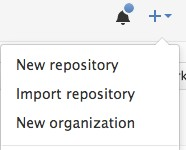
\includegraphics[scale=0.7]{figures/git.jpg}
    \label{git}
\end{figure}

Lengkapi	 data	 dan	 email	 kemudian	 Create	 Organization,	 kemudian	 masukkan	 username	anggota	untuk	kolaborasi dan	user	kordinator	proyek	2	awangga	sebagai	admin.	Setelah	itu	buat repository	 masing-masing	 anggota	 di	 dalam	 organisasi	 baru	 tersebut	 sesuai	 dengan	judul	proposal	masing-masing	sebagai	contoh	bisa	anda	buka	di \url{https://github.com/d4TI}

\begin{figure}[H]
    \centering
    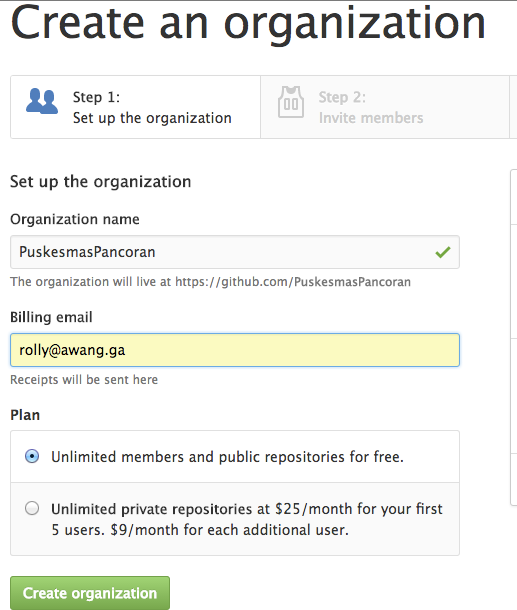
\includegraphics[scale=0.7]{figures/11.png}
    \label{11}
\end{figure}

Didalam	repositori	yang	didalamnya	terdapat	: \par 
\textbf{File	README.md} \par 
Berisi	 perkenalan	 diri	 nama,NPM,	 kelas,	 jurusan,	 kampus	 dan	 Judul	 dan	 deskripsi	 dari	Proyek	2	yang	diajukan	dalam	bahasa	Inggris	ditulis	dengan	script	markdown. \par 

\textbf{File	Licence} \par 
File	ini	dipilih	ketika	pertama	kali	repositori	dibuat. \par 

\textbf{Folder	doc} \par
Didalam	 folder	 doc	 ada	 folder	 proposal	 yang	 berisi	 tiga	 file	 isi	 dari	 proposal	 yaitu	abstraksi.md,	 BAB-I.md,BAB-II.md	 yang	 diisi	 dengan	 proposal	 peserta	 dalam	 bentuk	
markdown \par 

\textbf{Folder	img} \par 
Ini	adalah	folder	untuk	menaruh	gambar-gambar	yang	dimasukka	kedalam	proposal \par 

Pada	menu	Issues	peserta harus	mengisi	Milestone	dengan	jadwal-jadwal	penting	yang	ada	di	buku	petunjuk	ini.

\begin{figure}[H]
    \centering
    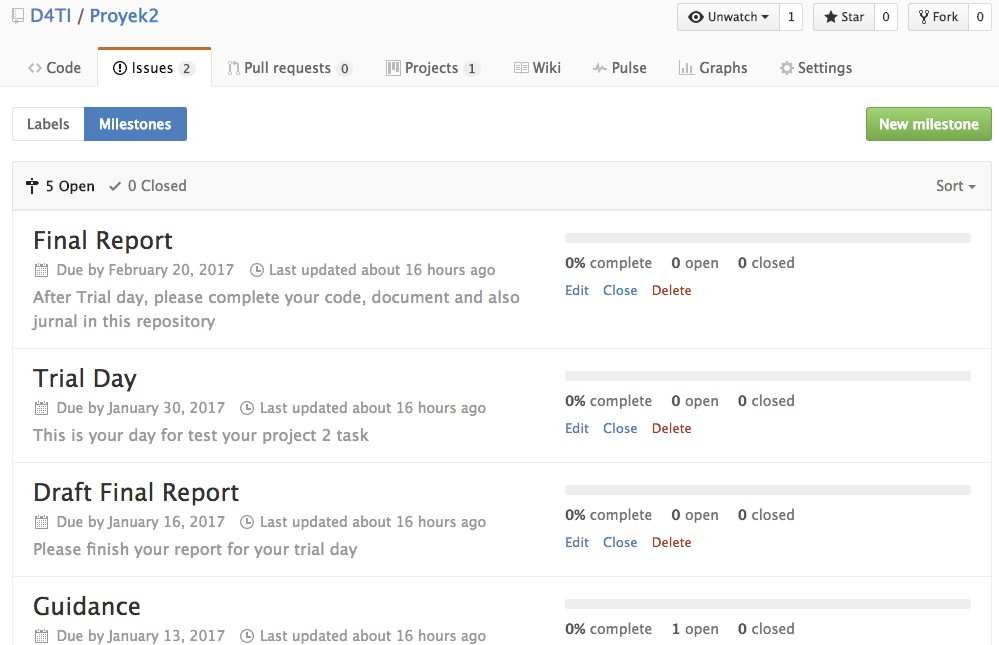
\includegraphics[scale=0.5]{figures/22.jpg}
    \label{22}
\end{figure}

Pada	menu	Project	peserta	membuat	New	Project	dengan	nama	Project	2	yang	didalamnya	berisi	Kanban	atau	scrum	dengan	kolom,	To	Do,	Doing,	Testing,	Done


\begin{figure}[H]
    \centering
    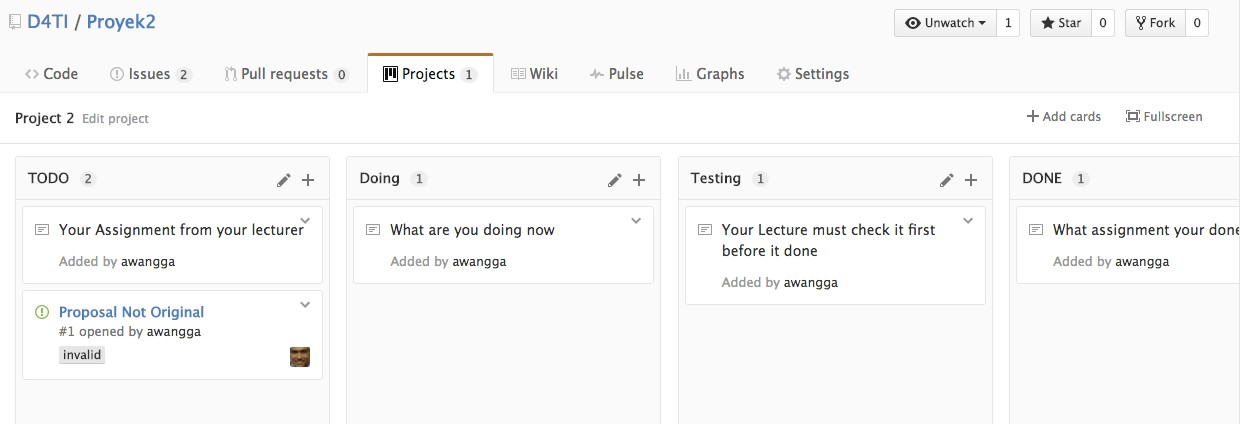
\includegraphics[scale=0.5]{figures/33.jpg}
    \label{33}
\end{figure}

Semua	 hasil	evaluasi	dan	 bimbingan(peserta	membantu	input	 sendiri	 hasil	 bimbingan) di	lempar	 ke	 menu	 issues dengan	 setting	 label	 sesuai	 dengan	 kriteria	 masalah,	 milestone	
sesuai	dengan	target	jadwal	yang	dikejar	assignment	untuk	ditujukan	kepada	peserta	yang	mana.	 Setelah	issues	masuk,	 kemudian	 oleh	 peserta	 dimasukkan	 ke	 kartu	 Scrum	 Todo	 di	menu	Project \textrightarrow Project	2dengan	klik	+Add	Cards. Ambil	kartu	yang	sedang	anda	kerjakan	pindahkan	ke	Doing,	setelah	selesai	masuk	ke	testing	begitu	seterusnya	hingga	kolom	To	Do	habis	 kartunya.	 Jika	pembimbing	menyetujui	pekerjaan	maka	 kartu	peserta	pindahkan	 ke	Done	dan	commit	file	yang	bersangkutan	dengan	menggunakan	hashtag	nomor	isu	agar	isu	
ter	 close	 secara	 otomatis(bukan	 di	 close	 dari	 tombol	 close	 di	 github).	 Semua	 perubahan	dan	 penambahan	 file	 di	 dalam	 repository \textbf{harus	 menggunakan	 aplikasi	 git	 bash} yang	standar	 sesuai	 dengan	 penjelasan	 di	 BAB	 selanjutnya,\textbf{dilarang	 keras	 melakukan	penambahan	 dan	 perubahan	 di	 web	 github	 secara	 langsung} dibuktikan	 dengan	perekaman	 pembuatan	 untuk	 disertakan	 di	 video	 log. Semua	 isi	 proposal	 di	 3	 file markdown \textbf{wajib	di	scan	plagiarism} 	hasil	screensot	plagiarisme	di	 taruh di	dalam	 folder	img/proposal dan	disertakan	link	tersebut	di	blog. Sebagai	contoh	repository	bisa	dilihat	di	
\url{https://github.com/D4TI/Proyek2/}.

\subsection{Video}
Peserta	juga	membuat	video	standar	sesuai	dengan	arahan	di	BAB selanjutnya.

\subsection{Blog}
Buat	 blog standar	 sesuai	 dengan	 arahan	 di	 BAB	 selanjutnya. Yang	 didalamnya	 sudah	diembed	video	dan	link	repository	serta	link	hasil	scan	plagiarism.
\\
\\
Proposal	di	submit	melalui	url	:
\\ \url{http://s.id/Proyek2}
\section{Reviewer}

\textit{Reviewer} adalah \textit{ team} yang	 terdiri	 dari	 2 orang	 yang	 mempunyai	 kepakaran	 di	 bidang	masalah	yang	akan	di	\textit{review}. \textit{\textbf{Team reviewer}} akan	ditunjuk	oleh	Koordinator	Proyek,	hasil evaluasi	yang	dilakukan	oleh \textit{\textbf{Reviewer}} adalah	mutlak,	dengan	ketentuan	sebagai	berikut	:

\begin{enumerate}
\item Dua Reviewer	menolak	maka	Proposal	Proyek	ditolak.
\item Satu Reviewer	menolak,	satu	menerima	maka	Proposal	Proyek	ditolak.
\item Dua Reviewer	menerima	maka	Proposal	Proyek	diterima.
\end{enumerate}

\section{Pengesahan	Proposal Proyek	II}
Persetujuan	 atas	 proposal	 oleh	 Koordinator	 Proyek	 II	 didasarkan	 pada	 hasil	\textit{Review} oleh \textit{Review},	yang	dibuktikan	dengan	diterbitkannya	surat	persetujuan	pelaksanaan	Proyek	II	kepada	 mahasiswa	 yang	 bersangkutan	 dan	 tembusan	kepada	 dosen	 pembimbing.	 Tanpa	surat	 persetujuan	 tersebut,	 pelaksanaan	 Proyek	 II	 bukan	 menjadi	 tanggung	 jawab Koordinator	Proyek II dan	tidak	akan	diproses	kelanjutannya.
\chapter{PENYUSUNAN LAPORAN}
\section{Tujuan}
Untuk	 melaporkan	 jalannya	 pekerjan	 Proyek	 serta	 hasil	 yang	 diperoleh,	 mahasiswa	diwajibkan	menyusun	laporan	pekerjaan	Proyek.

\section{Ketentuan Penyusunan Laporan}
\subsection{Format Laporan}
Laporan	Proyek	hendaknya	berisi	:

\begin{enumerate}
\item \textbf{ Bagian Awal}
	\begin{itemize}
		\item Lembar	Muka	
		\item Lembar Pengesahan
		\item Surat	Pernyataan	Tidak	Melakukan	Plagiarisme
	 \item Abstrak	(dalam	Bahasa	Indonesia)
	 \item Abstract(dalam	Bahasa	Inggris)
	 \item Kata	Pengantar
	 \item Daftar	Isi	termasuk	:
 \begin{enumerate}[label=(\alph*)]
 
	\item Daftar	Gambar
	\item Daftar	Tabel
	\item Daftar	Simbol
	\item Daftar	Singkatan	
	\item Daftar	Lampiran
 \end{enumerate}
 \end{itemize}
 
\item \textbf{Bagian Isi}
 	\par \textbf{BAB	I PENDAHULUAN}
 	
 	\begin{enumerate} [label=1.\arabic*]
 	\item \textbf{ Latar	Belakang} \par 
Berisi	ulasan	ringkas	mengenai	keadaan/kondisi	yang	ada	dan	
kekurangan	 dari	 sistem	 yang	 diamati	 sehingga	 muncul	 topik	
yang	diambil.

\item \textbf{ Identifikasi	Masalah} \par 
Berisi	 berbagai	 masalah	 yang	 sudah	 dikenali	 dan	 	 akan diberikan	 solusinya	 melalui	 fungsi	 dari	 sistem/aplikasi/alat	yang	akan	dibuat.

\item \textbf{Tujuan} \par
Berisi	tujuan	untuk	apa	sistem/aplikasi/alat	itu	dibuat.

\item \textbf{ Ruang	Lingkup	} \par
Berisi	batasan-batasan	proyek	atau	cakupan	aplikasi	yang	akan	
dibangun.

\item \textbf{ Sistematika	Penulisan} \par
Menjelaskan	isi	yang	ada	di	laporan	proyek.\\
 
 	\end{enumerate}
 	
 \par \textbf{BAB II LANDASAN TEORI} \par 
 
 	Uraian	 \textbf{tentang	 teori yang	 mendukung} Objek	 PROYEK 2.	 \textbf{Harus	jelas	 sumber	 rujukannya	 dari	 mana}. Sumber	 yang	 baik	 adalah	jurnal	 ilmiah,	 artikel	 ilmiah,	 buku,	 dll.	 \textit{\textbf{Disarankan	 untuk	 tidak	mengambil	sumber	seperti	WebBlog,	Wikipedia,	dll.}} \\
 	
 	\par \textbf{BAB III ANALISIS DAN PERANCANGAN} \par 
 	\textit{\textbf{Analisis}} : \par 
 	Proses	 untuk	 menentukan	 bentuk	 dari	 kebutuhan	
sistem/aplikasi/alat	 baik	 berupa	 kebutuhan	 pada	 saat	membangun	
maupun	pada	saat	Implementasi.

	\textit{\textbf{Perancangan}}: \par 
	Penjelasan	 perancangan	 	 sistem/aplikasi/alat	 	 yang	 akan	 dibuat	terdiri	dari	perancangan	alir	program \textit{\textbf{(Flow	Chart)}}	, algoritma,	data,	maupun	perancangan	input/output	sistem/aplikasi/alat.		
 	
	
	\begin{enumerate} [label=3.\arabic*]
		\item Analisis
			\begin{enumerate} [label=3.1.\arabic*]
				\item Analisis	Sistem	yang	Sedang	Berjalan
					\begin{enumerate} [label=3.1.1.\arabic*]
						\item Analisis	Prosedur/ \textit{Flow	Map} yang								  berjalan
						\item Analisis	Dokumen	yang digunakan
					\end{enumerate}
				\item Analisis	Sistem	yang	akan	Dibangun
					\begin{enumerate} [label=3.1.2.\arabic*]
						\item Analisis	Kebutuhan	Aplikasi
						\item Analisis	Kebutuhan	Perangkat	lunak									  dan	Perangkat Keras
					\end{enumerate}
			\end{enumerate}
			
			
		\item Perancangan \textit{\textbf{(Jika	menggunakan	procedural 					  atau DFD)}}
			\begin{enumerate} [label=3.2.\arabic*]
				\item \textit{Context	Diagram}
				\item \textit {Data	Flow	Diagram} (disertai	tabel									  spesifikasi	Proses)
				\item Kamus	Alir	Data \textit{(Data Dictionary)}
				\item 	Perancangan	 \textit{Database (Sesuaikan	Format							Penulisannya)}
					\begin{enumerate} [label=3.2.4.\arabic*]
						\item \textit{Conceptual	Data	Model}
						\item \textit{Physical	Data	Model}
						\item \textit{Kamus	Data	Tabel (Database)}	
					\end{enumerate}
				\item Struktur Menu
				\item Perancangan Antarmuka
			\end{enumerate}
			
	\end{enumerate}
			
			\begin{enumerate} [label=3.2]
				\item Perancangan \textit{\textbf{(Jika	menggunakan 							  	Object	Oriented UML)}}
			\end{enumerate}
				\begin{enumerate} [label=3.2.\arabic*]
				\item \textit{Use	Case	Diagram}
				\item \textit{Class	Diagram}
				\item \textit{Interaction	Diagram}
				\item \textit{Sequence	Diagram}
				\item \textit{Collaboration	Diagram}
				\item \textit{Activity	Diagram}
				\item \textit{Statechart	Diagram}
				\item \textit{Componen	Diagram}
				\item \textit{Deployment	Diagram}
				\item \textit{Objek	Diagram}
				\item Perancangan \textit{Database (Sesuaikan	Format							  Penulisannya)}
						\begin{enumerate}[label=(\alph*)]
							\item \textit{Conceptual Data Model	(CDM)}
							\item \textit{Physical	Data Model (PDM)}
						\end{enumerate}
				\item Struktur	Menu
				\item Perancangan	Antarmuka
				\end{enumerate} 
				
	\par \textbf{BAB IV IMPLEMENTASI DAN PENGUJIAN} \par 
	\textbf{Implementasi} : \par 
	adalah	sistem/aplikasi/alat	yang	dibuat	dengan	merinci	komponenkomponen	 pendukung	 berupa	 program,	 Lingkungan	 Implementasi, Tampilan	Antarmuka,	Petunjuk	Pemakaian,	Petunjuk	Instalasi.
	
	\textbf{Pengujian} : \par 
	Adalah	 Cara	 untuk	 mengetahui	 apakah	 sistem/aplikasi/alat	 yang dibuat	sesuai	dengan	rancangan	dan	menuliskan	hasil	ujinya.
\textit{Jika	 anda	 membuat	 analisis	 sistem/aplikasi,	 maka	 harus	 seperti berikut:}
	
	\begin{enumerate} [label=4.\arabic*]
		\item Lingkungan	Implementasi \par 	
		Berisi	 perangkat	 lunak	 dan	 perangkat	 keras	 apa	 saja yang	digunakan	 sewaktu	 perancangan	 aplikasi	 berupa	 sistem	operasi,	database,	prosesor,	memory,	space	harddisk	dan	lain-lain	sesuai	dengan	kebutuhan serta	perangkat	pendukungnya.
		
		\item Pembahasan	Hasil	Implementasi \par 
		Berisi	 uraian	 hasil	 implementasi	 sistem	 yang	 disesuaikan	dengan	 tujuan	 pembuatan	 sistem.	 Jelaskan bahwa	 masalah	 yang	teridentifikasi	 pada	 identifikasi	 masalah yang berada	 di	 bab	 1	 telah	terseleseaikan, dan	 tujuan	 dari	 pelaksanaan	 proyek	telah tercapai. Penjelasan	dibantu	dengan	Tampilan	Antarmuka	aplikasi.
		
		\item Pengujian	dan	hasil	Pengujian \par 
		Berisi	identifikasi	 pengujian,	 rencana	 pengujian,	 deskripsi dan hasil	uji.	Metoda	yang	digunakan	misalnya \textit{white	box testing} dan \textit{	black	box	testing}
		
	\end{enumerate}	 
	
	
	
	\par \textbf{BAB V KESIMPULAN	DAN	SARAN} \par 
	
	\begin{enumerate} [label=5.\arabic*]
		\item \textbf{Kesimpulan} : \par 
				berisi	pencapaian	tujuan	dari	sistem/aplikasi/alat	                yang	dibuat.
		\item \textbf{Saran} : \par 
				berisi	hal-hal	atau	tujuan	dari	pembuatan	sistem/aplikasi/alat	yang dirasa	belum	sempurna	atau	 tidak	 tercapai.	Saran	juga	bisa	berupa	kondisi	 implementasi	 yang	 optimal	 bagi	 sistem/aplikasi/alat	 yang dibuat.
	\end{enumerate}
			
			
\item Bagian Akhir
 \begin{itemize}
 	\item Daftar	Pustaka		(Lampiran	8)
 	\item Lampiran
 	\item Tabel-tabel
 \end{itemize} 
 		 	
\end{enumerate}

\section{Ukuran	Kertas	dan	Ukuran	Huruf}

\begin{itemize}
	\item Penulisan	 dan	 ejaan	 menggunakan	 ketentuan	 bahasa	 Indonesia	 yang	 baik	 dan	
benar;
	\item Penulisan	diketik	dengan	komputer,	dengan	ketentuan	:
		\begin{enumerate}
			\item Jarak	1,5 spasi ;
			\item Lebar	sembir	kiri	4	cm ;
			\item Lebar	sembir	kanan	2,5	cm ;
			\item Lebar	sembir	atas	3	cm ;
			\item Lebar	sembir	bawah	3	cm ;
			\item Ukuran	Font	adalah	\textit{Times	New	Roman} 12	Kecuali	untuk	judul	bab	menggunakan	\textit{Times New Roman} dengan	ukuran	14.
		\end{enumerate}
		
	\item Ukuran	buku	adalah	A4	(21	x	29,7	Cm),	dengan	berat	kertas	80	gram;
	
	\item Sampul	depan	adalah	mika/softcover mika,	dengan	ketentuan	seperti	ini	:
		\begin{enumerate}
			\item Proposal	Proyek   \qquad \qquad \enspace : Mika Transparan .
			\item Buku Laporan Proyek \qquad : \textit{Softcover} Merah Omega 17.
		\end{enumerate}
		
		
\section{Ketentuan	Khusus}
	\begin{enumerate}
		\item \textbf{Abstrak} : Jarak	 1	 spasi,	 maksimal	 1	 halaman,	 font	 12,	 italic,	 maksimum	 200	 kata.
Hanya	1	paragraf. Kata	kunci	minimal	5.

		\item Penomoran	 tabel	 dilakukan	 dengan	 menyebutkan	 nomor	 bab,	 diikuti	 nomor	 urut	tabelnya	pada	bab	tersebut,	misalnya	Tabel	3.7,	artinya	tabel	nomor 7	di	bab	3.	Judul	
tabel	 diletakkan	 di	 atas	 tabel,	 penulisannya	 dengan	 huruf	 kapital	 di	 awal	 kata.	 Bila	tabel	 lebih	 panjang	 dari	 halaman,	 maka	 sambungan	 tabel	 pada	 halaman	 berikutnya	
diberi	judul	dengan	tulisan	: \textbf{(Lanjutan)}
		\item Tulisan	di	dalam	tabel	Jarak	1 spasi,	ukuran	huruf kurang	atau	sama	dengan \textit{font} 10 ( $\leq \textit{font}  10$). 	Judul	tabel	disimpan diatas	table	tanpa	jarak	spasi.
		
		\item Penomoran	 gambar	 dilakukan	 dengan	menyebutkan	 nomor	 bab,	 diikuti	 nomor	 urut	gambarnya	pada	bab	tersebut,	misalnya		Gambar	2.5,	artinya	gambar	nomor	5	di	bab	
2.			 Judul	gambar	diletakkan	di	bawah	gambar,	penulisannya	dengan	huruf	kapital	di	awal	kata.

		\item Penomoran	 halaman	 dimulai	 dari	 nomor	 1	 untuk	 tiap	 bab	 atau	 lampiran,	 dengan	
ketentuan	sebagai	berikut:	\\
			Penomoran	 dari	 bab	 1	 sampai	 bab	 5	 dimulai	 dari	 halaman	 1	 sampai	 selanjutnya	sekuensial	tanpa	menggunakan	bab	contoh	;	pada	awal	bab	2,	jika	bab	1	sebanyak	10	halaman,	maka	bab	2	dimulai	dengan	halaman	11	dst. .
			
		\item Penomoran	 halaman	 judul,	 buku	 laporan,	 halaman	 	 persetujuan,	 Daftar	 Isi,	 Daftar	Tabel,	dan	Daftar		Gambar	menggunakan	i,		ii,		iii,	…..	(angka	romawi	kecil).
		
		\item Setelah	Buku	laporan	 ditandatangani	 oleh	 pembimbing	 dan	 penguji	 seminar/sidang,	
maka	harus	di	buatkan	Jurnal	dengan	jumlah	halaman	maksimum	6	halaman.

		\item \textit{Softcopy} dari	jurnal, \textit{software} dan	laporan	disimpan	dalam	sebuah	CD	dan	disertakan	
ke	dalam	laporan di	beri	judul	serta	penulis	di	label	CD	nya.

	\end{enumerate}
\end{itemize}

\section{Status	Buku}
\begin{enumerate}
	\item Status Buku \par 
		Buku	 yang	 memenuhi	 persyaratan	 untuk	 sidang Proyek	 adalah	 buku	 yang	 telah	
selesai	 100 \%.	 Penjilidan	 buku	 sebelum	 sidang menggunakan	 penjepit	 dan	 sampul	plastik	mika	warna	Transparan;

	\item Setelah	Sidang \par 
		Buku	 yang	 memenuhi	 persyaratan	 untuk	 keluarnya	 nilai	 adalah	 buku	 yang	 telah	selesai	 100 \%	 (telah	 diperbaiki,	 jika	 ada	 tugas	 perbaikan).Penjilidan	 	 buku	 setelah	sidang dan	 setelah	 melalui	 perbaikan	 adalah	 jilid	 punggung	 disertai	 halaman	pembatas	bab	warna	merah	seperti	pita	pembatas	warna	merah.	
		
\end{enumerate}

\section{Distribusi	Buku}
Jumlah	 salinan	 laporan	 Proyek	 untuk	 keperluan	 sidang Proyek	 adalah	 3	 \textit{copy},	 dengan	distribusi	sebagai	berikut	:

\begin{enumerate}
	\item Pembimbing/Ketua	Penguji \quad (1 copy)
	\item Anggota	Penguji \qquad \qquad \qquad(1 copy)
	\item Mahasiswa \qquad \qquad \qquad \enspace \quad \quad(1 copy)
\end{enumerate}

Jumlah	salinan	buku	laporan	Proyek		adalah	4	 (empat) \textit{	 copy},	dengan	distribusi	sebagai	berikut	:

\begin{table}[H]
\label{tab:my-table}
\begin{tabular}{lll}
1 & Pembimbing & (1 CD) \\ \\
2 & Perpustakaan	Politeknik	Pos	Indonesia & (1 Buku dan CD ) \\ \\
3 & Mahasiswa & (1 Buku) \\ \\
4 & \multicolumn{2}{l}{\begin{tabular}[c]{@{}l@{}}Prodi	(1	 CD yang	 berisi	 jurnal,	 aplikasi	 dan	 laporan) dan	 hardcopy	 jurnal	 1	 buah	\\ tanpa	di	jilid.\end{tabular}}
\end{tabular}
\end{table}

\chapter{SIDANG PEKERJAAN PROYEK II}
\section{Tujuan}
Untuk	menguji	mahasiswa	atas	pekerjaan	Proyek II yang	 telah	dikerjakan	maka	diadakan	
sidang Proyek II.

\section{Waktu}
Sidang Proyek	diselenggarakan	pada	waktu	yang	telah	ditentukan	dan	diatur	pada	Petunjuk	
Pelaksana.

\section{Syarat	Sidang}
Proyek	yang	diajukan	ke	Sidang Proyek II adalah	Proyek	yang	telah	memenuhi	persyaratan	
sebagai	berikut	:

\begin{enumerate}
	\item Nilai	bimbingan	$ \geq80$ untuk	masing-masing	pembimbing .
	\item Aplikasi,	Sistem	atau	Alat	yang	dibuat	telah	selesai	$\geq90\%$ .
	\item Buku	laporan	telah	terselesaikan	100\% .
	\item Buku	 laporan	 telah	 diserahkan	 ke	 penguji	 paling	 lambat	 2	 minggu sebelum	 hari	
pelaksanaan	Sidang Proyek II .
	\item Diijinkan	sidang oleh	pembimbing,	dibuktikan	dengan	surat	permohonan	sidang Proyek
II .
	\item Telah	mendapat	nilai	Bimbingan	dari	pembimbing .
	\item 2	Minggu	sebelum	sidang	sudah	memberikan	laporan	ke	pembimbing,	jika	pembimbing	
berhalangan	segera	konfirmasikan	ke	koordinator	proyek.
	\item Sudah	melunasi	SPP.
	\item Mendaftarkan	sidang	ke	koordinator	proyek.
\end{enumerate}

\section{Penguji}
	\subsection{Penentuan Penguji}
		Penguji	ditentukan	oleh	Koordinator	Proyek	II	dan	penunjukannya	disampaikan	dengan	
diterbitkannya	surat	keputusan	tentang	pembentukan	panitia	sidang Proyek II.
	\subsection{Jumlah Penguji}
	Jumlah	penguji	adalah dua	orang. Yang	terdiri	dari	Ketua	Penguji	dan	anggota	penguji.
Ketua	Penguji		adalah	Pembimbing	Proyek II ,	dan	anggota	penguji	adalah	penguji	yang	
ditunjuk	 oleh	 koordinator	 yang	 kedua	 duanya	 disampaikan	 dengan	 surat	 keputusan.	
Sidang dengan	penguji	kurang	dari	2	orang	dianggap	batal.
	\subsection{Susunan	panitia	Sidang Proyek II}
	\begin{itemize}
		\item Ketua Penguji
		\item Anggota
	\end{itemize}
	
\section{Penilaian}
\begin{enumerate}
	\item Kriteria	penilaian	adalah	sesuai	dengan \textit{form} penilaian.
	\item Penilaian	menggunakan	angka	1-100 dengan	kategori	sebagai	berikut
		\begin{enumerate}[label=(\alph*)]
		\item \textit{Design	Antar	Muka}.
		\item Implementasi web	 service	 dengan	 Oauth	 2	 atau	 				  sistem	 token	 antara	\textit{Client/Servernya}.
		\item Bahasa	Pemograman	menggunakan	framework.
		\item Seluruh	 table	 diisi	 dengan	 data	 dummy	 sebanyak	 satu	 juta	 record	 masing-masing	 ketika	demo	 sidang, database	juga	menggunakan	procedure,	 fungsi	dan atau trigger. Implementasikan	juga \textbf{redis} sebagai	database	cache
		\item Study Kasus.
		\end{enumerate}
\end{enumerate}

\section{Kehadiran Pembimbing}
	Sidang tanpa	kehadiran	pembimbing	dianggap	BATAL	dan	pelaksanaannya	akan	ditentukan	
kemudian.

\section{Persyaratan	Administrasi	Sidang}
	Sebelum	sidang harus	tersedia \textit{form-form} yang	diperlukan	yaitu	:
	\begin{enumerate}
		\item Berita	Acara	Sidang
		\item Lembar	catatan/perbaikan	Proyek	
		\item Lembar	penilaian	sidang Proyek
		\item Lembar	persyaratan	untuk	lulus	bersyarat	
		\item Lembar	penilaian	bimbingan	
	\end{enumerate}
	\par \textit{Form} tersebut	 diatas	 harus	 sudah	 ada	 pada	 peguji	 sidang	 proyek	 sebelum	 sidang	 itu	
dimulai.

\section{Status	Hasil	Sidang Proyek}
Status	hasil	sidang Proyek	adalah	sebagai	berikut	:
\begin{enumerate}
\item Lulus.
\item Lulus Bersyarat.
\item Tidak Lulus.
\end{enumerate}
\par Status	tersebut	ditentukan	oleh	sidang	dewan	penguji
\chapter{KRITERIA HASIL SIDANG}

\section{Lulus}
Mahasiswa	dinyatakan	lulus	sidang Proyek	jika	:
\begin{enumerate}
	\item Menjalani	sidang dengan	lancar.
	\item Tidak	terjadi	revisi,	baik aplikasi	maupun	laporan	proyek.
	\item Mendapat	nilai	dengan	rata-rata	dari	penguji	minimum	60.	
\end{enumerate}

\section{Lulus Bersyarat}
Mahasiswa	dinyatakan	lulus	bersyarat	dari	sidang Proyek	jika	:
\begin{enumerate}
\item Memenuhi	persyaratan	lulus.
\item Ada	 tugas	 yang	 diberikan	 penguji,	 jika	 tugas	 tersebut	 	 telah	 selesai	 dikerjakan	 maka	
statusnya	otomatis	berubah	menjadi	Lulus.	\\
Tugas	tersebut	berupa	:
\begin{itemize}
\item Perbaikan Laporan.
\item Perbaikan Aplikasi.
\end{itemize}
\end{enumerate}

\section{Tidak Lulus}
Mahasiswa	dinyakan	tidak	lulus	sidang Proyek	jika	:
\begin{itemize}
\item Ditemukan	hasil \textit{plagiat} 80\%	dari	Proyek	I,	II	yang	pernah	disidangkan.
\item Tidak	memenuhi	kriteria	Lulus.
\item Tidak	datang	pada	waktu	sidang	 tanpa	informasi	apapun,	sedangkan	 tim	penguji	sudah	siap	di	lokasi	sidang.
\end{itemize}

\section{Penilaian}
\subsection{Komponen	Nilai}
Nilai	Proyek	tersedia	atas	dua	komponen	nilai yaitu	:
\begin{itemize}
	\item Nilai	buku	dan	bimbingan.
	\item Nilai	sidang Proyek.
\end{itemize}

\subsection{Nilai	Buku	dan	Bimbingan}
Nilai	buku	dan	bimbingan	dikeluarkan	oleh	pembimbing,	dengan	skala	nilai	1-100. Nilai	
akhir	buku	dan	bimbingan	adalah	nilai	rata-rata	dari	seluruh	pembimbing.Paling	lambat	2	
hari	 sebelum	 sidang,	 mahasiswa	 wajib	 menyerahkan	 nilai	 dari	 pembimbing	 ke	
koordinator	proyek.

\subsection{Nilai	Sidang Proyek	Pemrograman	dan	Jaringan (PROYEK	II).}
Nilai	 ini	 dikeluarkan	 oleh	 penguji,	 dengan	 skala	 nilai	 1-100	 segera	 setelah	 sidang
dilaksanakan,	 ketua	 sidang wajib	 menyerahkan	 hasil	 penilaiannya.Nilai	 Proyek	 adalah	
35\%	dari	rata-rata	nilai	pembimbing	dan	65\%	dari	rata-rata	nilai	Penguji.

\subsection{Pengolahan	Nilai}
Pengolahan	 nilai	 dilaksanakan	 oleh	 Koordinator	 Proyek.	 Dalam	 menjalankan	 tugas	pengolahan	nilai,	Koordinator	Proyek	mempunyai	hak	penuh	 yang	 tidak	dapat	diganggu	
gugat	 oleh	 siapa	 pun.	 Pengolahan	 nilai	 dilaksanakan	 berdasarkan	 nilai	 yang	 diberikan	
oleh	pembimbing	dan	penguji	sidang Proyek.	Adapun	rumus	yang	dipakai	adalah	sebagai	
berikut	: \\

\textbf{Nilai	Akhir	=			(35\%	x	rata-rata	nilai	bimbingan)	+	(65\% x	rata-rata	nilai	sidang)	} \\

\textbf{Index Nilai :} \\
$85	\leq Nilai	\leq 100$	= A \\
$71	\leq Nilai	\leq 84$	= B \\
$56	\leq Nilai	\leq 70	$	= C \\

\subsection{Distribusi	Hasil	Pengolahan	Nilai}
Nilai	 Proyek	 Program	 disampaikan	 ke	 mahasiswa	 yang	 bersangkutan	 dan	 Ketua	 Prodi oleh	 Koordinator	 Proyek.	 Nilai	 tersebut	 akan	 keluar,	 jika	 persyaratan	 keluarnya	 nilai	Proyek	 telah	 terpenuhi.	 Koordinator	 Proyek	 mempunyai	 hak	 penuh	 untuk	 tidak	mengeluarkan	nilai	Proyek	jika	mahasiswa	 tidak	memenuhi	persyaratan	keluarnya	nilai	Proyek.	Adapun	nilai	Proyek	akan	dikeluarkan	oleh	Koordinator	Proyek	jika	:
\begin{enumerate}
	\item Buku	telah	dijilid	dan	didistribusikan	sesuai	dengan	ketentuan.
	\item . Tidak		ada			permasalahan		dengan		pinjaman		fasilitas	dan	alat	yang	digunakan	selama	
pelaksanaan	Proyek .
	\item Menyerahkan	 alat	 hasil	 Proyek	 bagi	 mahasiswa	 yang	 telah	 menyatakan	 kesediaanya	untuk	menyumbangkan	alat	tersebut .
	\item Mengumpulkan	CD	Proyek .
	\item Mengumpulkan	Jurnal Proyek	dalam	bahasa	Indonesia	dan	Inggris.	
\end{enumerate}
\chapter{PENGELOLAAN APLIKASI, SISTEM ATAU ALAT HASIL PEKERJAAN
PROYEK, JURNAL, DAN FOTO ALAT}

\section{Tujuan}
Aplikasi,	 Sistem	 atau	 Alat	 hasil	 pekerjaan	 Proyek	 sangat	 berguna	 bagi	 pengembangan	
laboratorium	 dan	 kualitas	 Proyek	 karena	 itu	 pengelolaannya	 harus	 benar-benar	
dilaksanakan.Begitu	juga	dengan	abstrak,	dan	foto	alat.

\section{Perangkat Lunak}
Pengelolaan	 alat	 atau	 perangkat	 lunak	 diserahkan	 ke	 Prodi	 D4,	 dan	 menjadi tanggung	
jawab	Ketua	Prodi.

\section{Jurnal}
Abstrak	 didokumentasikan	 oleh	 Koordinator	 Proyek	 dan	menjadi	 bahan	 penerbitan	 buku	Jurnal Proyek,	 yang	 diterbitkan	 setahun	 sekali	 oleh	 Prodi.	 Dengan	 penerbitan	 buku	
tersebut,	 diharapkan	 tidak	 ada	 terjadi	 dua	 Proyek	 dengan	 topik	 yang	 sama,	 diharapkan	juga	kualitas	Proyek	dapat	terpantau	melalui	buku	ini.

\section{Syarat Khusus}
Semua	perangkat	lunak	harus	dapat	diakses	melalui	jaringan.	Jika	Aplikasi	berbasis	:
\begin{itemize}
\item Desktop	harus	dijalankan	tanpa	debugger	(contoh:	visual	studio).
\item Mobile	harus	 dijalankan	di	perangkat	sebenarnya	bukan	emulator.
\item Web	alamat	url	tidak	boleh	terlihat	localhost.
\item Gunakan	fitur	web	service.
\item Perhatikan	masalah	keamanan	jaringan.
\end{itemize}

\chapter{CARA MERUJUK DAN MENULIS DAFTAR RUJUKAN (PUSTAKA)}
Pembuatan	daftar	pustaka \textbf{diwajibkan} menggunakan	 fitur	Reference	Bibiliography	di	Microsoft Office	sehingga	daftar	pustaka	tercipta	dengan	otomatis.\\
Cara	merujuk	daftar	pustaka	adalah	sebagai	berikut:
\begin{enumerate}
\item Daftar	Pustaka	disusun	menurut	urutan	kutipan	dan	diberi nomor	urut	mulai	dari	[1].
\item Judul	buku	tidak	boleh	disingkat.
\item Penyingkatan	kependekan	Jurnal	Ilmiah	harus	mengikuti	yang	telah	lazim	dilakukan.
\item Nama	keluarga	(nama	belakang)	ditulis	terlebih	dahulu,	diikuti	dengan	singkatan	nama	depan.
\item Semua	nama	pengarang	harus	ditulis	sesuai	dengan	urutannya	di		dalam	artikel	/	buku.
\end{enumerate}

\par Penjelasan	lebih	rinci	mengenai	cara	merujuk	dan	menulis	daftar	rujukan	dijelaskan	sebagai	
berikut

\section{Cara	Merujuk}
Perujukan	 dilakukan	 dengan	menggunakan	 nama	 	 akhir	 dan	 tahun	 di	 antara	 tanda	 kurung. Jika	ada	dua	penulis,	perujukan	dilakukan	dengan	cara	menyebut	nama	akhir	kedua	penulis	
tersebut.	Jika	penulisnya	lebih	dari	dua	orang,	penulis	rujukan	dilakukan	dengan	cara	penulis	nama	pertama	dari	penulis	 tersebut	diikuti	dengan \textit{dkk}. Jika	nama	penulis	 tidak	disebutkan,	yang	 dicantumkan	 dalam	 rujukan	 adalah	 nama	lembaga	 yang	menerbitkan,	 nama	 dokumen yang diterbitkan,	 atau	 nama	 koran.	 Untuk	 karya	 terjemahan,	 perujukan	 dilakukan	 dengan	cara	menyebutkan	nama	penulis	aslinya.	Rujukan	dari	dua	sumber	atau lebih	yang	ditulis	oleh penulis	yang	berbeda	dicantumkan	dalam	satu	tanda	kurung	dengan	titik	koma	sebagai	tanda	pemisahnya.

\section{Cara	Merujuk	Kutipan	Langsung}
\subsection{Kutipan	Kurang	dari	40	Kata}
Kutipan	 yang	 berisi	 kurang	 dari	 40	 kata	 ditulis	 di	 antara	 tanda	 kutip	 (“…”)	 sebagai	bagian	 yang	 terpadu	 dalam	 teks	 utama,	 dan	 diikuti	 nama	 penulis,	 tahun	 dan	 nomor	halaman.	 Nama	 penulis	 dapat	 ditulis	 secara	 terpadu	 dalam	 teks	 atau	 menjadi	 satu	dengan	tahun	dan	nomor	halaman	di	dalam	kurung.	Lihat	contoh	berikut. Nama	penulis disebut	dalam	teks	secara	terpadu \\
\\

\textbf{Contoh :}\\
Tersine	 (1994:	 28)	 menyatakan	 “tekanan	 pasar	 memaksa	 organisasi	 untuk	menghasilkan	produk	yang	lebih	beragam	dan	kemampuan	pengiriman	yang	lebih	baik” Nama	penulis	disebut	bersama	dengan	tahun	penerbitan	dan	nomor	halaman.
\\
\\

\textbf{Contoh :}\\
Hal	 tersebut	 berdasarkan	 pada	 pernyataan	 “tekanan	 pasar	memaksa	 organisasi	 untuk	menghasilkan	produk	yang	lebih	beragam	dan	kemampuan	pengiriman	yang	lebih	baik”	
(Tersine,	1994:28). \\
Jika	ada	tanda	kutip	dalam	kutipan,	digunakan	tanda kutip	tunggal	(‘…’).
\\
\\

\textbf{Contoh :}\\
Ini	sejalan	dengan	pernyataan	Bickelhaupt	yang	menyatakan	“Kontrak	asuransi	bersifat	pribadi	 (personal)	 dang	 ‘mengikuti’	 pribadi	 itu,	 bukan	 ‘mengikuti’	 harta	 yang	diasuransikan.”

\subsection{Kutipan	40	Kata	atau	Lebih}
Kutipan	yang	berisi	40	kata	atau	lebih	ditulis	tanpa	tanda	kutip	secara	terpisah	dari	teks	yang	mendahului,	 ditulis	 1,2	 cm	 dari	 garis	 tepi	 sebelah	 kiri	 kanan,	 dan	 diketik	 dengan	spasi	tunggal.	Nomor	halaman	juga	harus	ditulis.
\\
\\
\\
\textbf{Contoh :}\\
Harrington	 (1999	 :	 384)	 menarik	 kesimpulan	 sebagai	 berikut.“Making	 manufacturers	strictly	liable	for	all	consumer	losses	can	improve	safety	incentives	when	consumers	are	
uninformed	 about	 product	 risk,	 because	 strict	 liability	 gives	 manufacturers	 proper	incentives	 to	make	safe	products	and	induces	consumers	 to	purchase	 the	right	amount	of	risky	products.” \\
Jika	dalam	kutipan	 terdapat	paragraf	baru	lagi,	garis	barunya	dimulai	1,2	cm	dari	 tepi	
kiri	garis	teks	kutipan.

\subsection{Kutipan	yang	Sebagian	Dihilangkan}
Apabila	 dalam	 mengutip	 langsung	 ada	 kata-kata	 dalam	 kalimat	 yang	 dibuang,	 maka	kata-kata	yang	dibuang	diganti	dengan	tiga	titik. \\
\\

\textbf{Contoh :}\\
"Asuransi	konstruksi	menjamin	kerugian	akibat	kerusakan	fisik	pada	proyek	pekerjaan	teknik	sipil	…	disebabkan	kecelakaan	yang	terjadi	pada	masa	pembangunan.” \\

Apabila	ada	 kalimat	 yang	 	 dibuang,	maka	 kalimat	 yang	 dibuang	 diganti	 dengan	empat	titik.\\
\\

\textbf{Contoh :}\\
“Kerugian	 tidak	langsung	juga	 timbul	pada	bangunan	 yang	 tidak	memenuhi	 ketentuan	sehingga	harus	dilakukan penggantian	semua	atau	sebagian	bangunan	tersebut	….Maka	kerugian	 tak	 langsung	 ada	 berupa	 biaya	 membuka	 bagian	 yang	 tidak	 salah,	 nilai	 dari	bagian	yang	tidak	dirusakkan,	dan	perbedaan	nilai	bangunan	setelah	diperbaiki	dengan	nilai	bangunan	sebelumnya”	(Darmawi,	2000:144).

\subsection{Cara	Merujuk	Kutipan	Tidak	Langsung}
Kutipan	 yang	 disebutsecara	 tak	 langsung	 atau	 dikemukakan	 dengan	 bahasa	 penulis	 sendiri	ditulis	tanpa	tanda	kutip	dan	terpadu	dalam	teks.	Nama	penulis	bahan	kutipan	dapat	disebut	terpadu	 dalam	 teks,	 atau	 disebut	 dalam	 kurung	 bersama	 tahun	 penerbitannya.	 Jika	memungkinkan	nomor	halaman	disebut	terpadu	dalam	teks.
\\
\\
\textbf{Contoh :} \\
Skipper	 (1999:453)	 hanya	 melakukan	 peramalan	 permintaan	 dengan	 pendekatan	 regresi	linier.\\ Nama	penulis	disebut	dalam	kurung	bersama	tahun	penerbitannya.\\
\textbf{Contoh :}\\
Untuk	kasus	tersebut,	regresi	logistik	ternyata	memberikan	hasil	yang	lebih	baik	(Wolff,	2000	
:	144).

\subsection{Cara	Menulis	Daftar	Rujukan (Pustaka)}
Daftar	rujukan	merupakan	daftar	yang	berisi	buku,	makalah,	artikel,	atau	bahan	lainnya	yang	dikutip	 baik	 secara	 langsung	 maupun tidak	 langsung.	 Bahan-bahan	 yang	 dibaca	 akantetapi	tidak	dikutip	\textit{tidak	dicantumkan} 	dalam	daftar	rujukan,	sedangkan	semua	bahan	yang	dikutip	secara	langsung	ataupun	 tak	langsung	dalam	 teks \textit{harus} dicantumkan	dalam	daftar	 rujukan.	

Pada	 dasarnya,	 unsur	 yang	 ditulis	 dalam	 daftar	 rujukan	 secara	 berturut-turut	 	meliputi	 (1)	nama	penulis	ditulis	dengan	urutan	:	nama	akhir,	nama	awal,	dan	nama	 tengah,	 tanpa	gelar	akademik,	 (2)	 tahun	 penerbitan,	 (3)	judul,	 termasuk	 anak	judul	(\textit{subjudul}),(4)	 kota	 tempat	
penebitan,	 dan	 (5)	 nama	 penerbit.	 Unsur-unsur	 tersebut	 dapat	 bervariasi	 tergantung	 jenis	sumber	 pustakanya.	 Jika	 penulisnya	 lebih	 dari	 satu,	 cara	 penulisan	 namanya	 sama	 dengan	penulis	pertama	(Lampiran-8). \\

Nama	 penulis	 yang	 terdiri	 dari	 dua	 bagian	 ditulis	 dengan	 urutan:	 nama	 akhir	 diikuti	 koma,	nama	 awal	 (disingkat	 atau	 tidak	 disingkat	 tetapi	 harus	 konsisten	 dalam	 satu	 karya	ilmiah), diakhiri	dengan	 titik.	Apabila	sumber	yang	dirujuk	ditulis	oleh	lain,	semua	nama	penulisnya	harus	dicantumkan	dalam	daftar	rujukan.
\\
\\

\textbf{Rujukan dari Buku} \par


Tahun	 penerbitan	 ditulis	 setelah	 nama	 penulis,	 diakhiri	 dengan	 titik.	 Judul	 buku	 ditulis	dengan	 huruf	 miring,	 dengan	 huruf	 besar	 pada	 awal	 setiap	 kata,	 kecuali	 kata	
hubung.Tempat	penerbitan	dan	nama	penerbit	dipisahkan	dengan	titik	dua	(:). \\
\\
\textbf{Contoh :} \\
Magee,	J.	F.	\&	Boodman,	D.	M.	1967. \textit{Production	Planning	and	Inventory	Control.}	New	York: McGraw-Hill. \\
Jika	 ada	 beberapa	 buku	 yang	 dijadikan	 sumber	 ditulis	 oleh	 orang	 yang	 sama	 dan	diterbitkan	dalam	tahun	yang	sama	pula,	data	tahun	penerbitan	diikuti	oleh	lambang	a,	b,	
dan	 c,	 dan	 seterusnya	 yang	 urutunnya	 ditentukan	 secara	 kronologis	 atau	 berdasarkan	abjad	judul	buku-bukunya. \\
\\

\textbf{Contoh :} \\
Cummins,	J.	D.	1992a. \textit{Should	Automobile	Insurance	be	Compulsary?}	Cincinnati,	OH:	General	Publisher. \\
Cummins,	 J.	 D.	 1992b.	\textit{Should	 Automobile	 Insurance	 be	 Compulsary:	 The	 Second	Perspective}. Cincinnati,	OH:	General	Publisher.
\\
\\
\textbf{Rujukan dari Buku yang Berisi Kumpulan Artikel (Ada Editornya)}


Seperti	menulis	rujukan	dari	buku	ditambah	dengan	tulisan	(Ed.)	jika ada	satu	editor	dan	(Eds.)	jika	editornya	lebih	dari	satu,	di	antara	nama	penulis	dan	tahun	penerbitan. \\ \\

\textbf{Contoh :}
Park,	S.	\&	Browse,	R.	(Eds.).	1998. \textit{A	Text	on	Marine	Insurance}.	New	York:	Pogue. \\
Dijkstra	(Ed.).	1990. \textit{Logistics Management}. New	York:	The	Foundation	Presss.
\\
\\
\textbf{Rujukan dari Artikel dalam Buku Kumpulan Artikel (Ada Editornya)}


Nama	penulis	artikel	ditulis	di	depan	diikuti	dengan	tahun	penerbitan.	Judul	artikel	ditulis	tanpa	 cetak	 miring.	 Nama	 editor	 ditulis	 seperti	 menulis	 nama	 biasa,	 diberi	 keterangan	(Ed.)	bila	hanya	satu	editor,	dan	(Eds.)	bila	lebih	dari	satu	editor.	Judul	buku	kumpulannya	ditulis	dengan	huruf \textit{miring}, dan	nomor	halamannya	disebutkan	dalam	kurung.\\
\\
\textbf{Contoh :}\\
Hartley,	 J.T.,	Harker,	 J.O.	\&	Walsh,	D.A.	1980. Contemporary	 Issues	and	New	Directions	in	Adult	 Development	 of	 Learning	 and	Memory.	 Dalam	 L.W.	 Poon	 (Ed.) \textit{Aging	in	 the	 1980s:	Psychological	Issues}(hlm.	239-252).	Washington,	D.C.:	American	Psycological	Association.\\
 Hasan,	 M.Z.	 1990.	 Karakteristik	 Penelitian	 Kualitatif.	 Dalam	 Aminuddin	 (Ed.),\\ \textit{Pengembangan	Penelitian	Kualitatif	dalam	Bidang	Bahasa	dan	Sastra} (hlm.	12-25).	Malang:	HISKI	Komisariat	Malang	dan	YA3.
 \\
 \\
 \textbf{Rujukan dari Artikel dalam Jurnal}\\
 Nama	 penulis	 ditulis	 paling	 depan	 diikuti	 dengan	 tahun	 dan	 judul	 artikel	 yang	 ditulis	dengan	 cetak	 biasa,	 dan	 huruf	 besar	 pada	 setiap	 awal	 kata.	 Nama	 jurnal	 ditulis	 dengan	cetak	miring,	 dan	 huruf	awal	 dari	 setiap	 katanya	 ditulis	 dengan	 huruf	 besar	 kecuali	 kata	hubung.	Bagian	akhir	berturut-turut		ditulis		jurnal	tahun	keberapa,	nomor	berapa	(dalam	kurung),	dan	nomor	halaman	dari	artikel	tersebut.\\
\\
\textbf{Contoh :}\\
Wuhrer,	 J.	 1975.	Better	Group	 Corporate	Health	 Financing.	\textit{Journal	 of	Risk	 and	 Insurance}, 1(3):	47-50.
\\
\\
\textbf{Rujukan dari Artikel dalam Jurnal dari CD-ROM}
Nama	penulis	ditulis	paling	depan,	diikuti	oleh	 tanggal,	bulan,	dan	 tahun	(jika	ada).	 Judul	artikel	ditulis	dengan	cetak	biasa,	dan	huruf	besar	pada	setiap	huruf	awal	kata,	kecuali	kata	
sambung.	Nama	majalah	ditulis	dengan	huruf	kecil	kecuali	huruf	pertama setiap	kata,	dan	dicetak \textit{miring}. Nomor	halaman	disebut	pada	bagian	akhir.
\\
\\Suryana,	 1996.	 Optimalisasi	 Waktu	 Perjalanan	 dengan	 Translasi	 Nonlinier. \textit{Jurnal	Transportasi},	3(3):55-59.
\\
\\
\textbf{Rujukan dari Koran Tanpa Penulis}
\\
Nama		koran	ditulis	di	bagian	awal.	Tanggal,	bulan,	dan	tahun	ditulis	setelah	nama	koran,	
kemudian	judul	ditulis	dengan	huruf	besar-kecil	dicetak	miring	dan	diikuti	dengan	nomor	halaman.
\\
\\
\textbf{Contoh :}
Suara	Pembaruan.	26	Juni,	1998. \textit{Asuransi	Perjalanan	Wisata},	5.	
\\
\\
\textbf{Rujukan dari Lembaga yang Ditulis Atas Nama Lembaga Tersebut}
\\
Nama	 lembaga	 penanggung	 jawab	 langsung	 ditulis	 di	 depan,	 diikuti	 dengan	 tahun,	 judul	karangan	 yang	 dicetak	 miring,	 nama	 tempat	 penerbitan,	 dan	 nama	 lembaga	 yang	bertanggung	jawab	atas	penerbitan	karangan	tersebut.
\\
\\
\textbf{Contoh :}
\\
Dewan	Asuransi	Indonesia.	1989. \textit{Perkembangan	Bisnis	Asuransi	di	Indonesia	Periode}	1975-1985.	Jakarta:	Dewan	Asuransi	Indonesia.
\\
\\
\textbf{Rujukan Berupa Karya Terjemahan}\\
Nama	 penulis	asli	 ditulis	 di	 depan,	 diikuti	 tahun	 penerbitan	 karya	asli,	judul	 terjemahan,	nama	 penerjemah,	 tahun	 terjemahan,	 nama	 tempat	 penerbitan	 dan	 nama penerbit	terjemahan,.	 Apabila	 tahun	 penerbitan	 buku	 asli	 tidak	 dicantumkan,	 ditulis	 dengan	 kata \textit{Tanpa	tahun}.
\\
\\
\textbf{Contoh :} \\
Zaelani,	 G.	 1989. \textit{Suatu	 Tinjauan	 tentang	 Ukuran-ukuran	 Efisiensi	 Sistem	 Transportasi}.	Skripsi	tidak	diterbitkan.	Jakarta:	Universitas	Trisakti.
\\
\\
\textbf{Rujukan Berupa Makalah yang Disajikan dalam Seminar, Penataran, atau Lokakarya}
\\
Nama penulis ditulis paling depan, dilanjutkan dengan tahun, judul makalah ditulis dengan cetak miring, kemudian diikuti pernyataan “Makalah disajikan dalam ..”., nama pertemuan, lembaga penyelengara, tempat penyelenggaraan, dan tanggal serta bulannya.
\\
\\
\textbf{Contoh :}
\\
Huda,	 N.	 1991. \textit{Penulisan	 Laporan	 Penelitian	 untuk	 Jurnal}.	 Makalah	 disajikan	 dalam	Lokakarya	Penelitian	Tingkat	Dasar	bagi	Dosen	PTN	dan	PTS	di	Bandung,	Pusat	Penelitian	IKIP	Malang,	Malang,	12	Juli. 
\\
Karim,	Z.	1987. \textit{Tatakota	di	Negara-negara	Berkembang}. Makalah	disajikan	dalam	Seminar	Tatakota,	BAPPEDA	Jawa	Timur,	Surabaya,	1-2	September.
\\
\\
\textbf{Rujukan dari Internet berupa Karya Individual}
\\
Nama	penulis	ditulis	seperti	rujukan	dari	bahan	cetak,	diikuti	secara	berturut-turut	oleh	tahun,	 judul	 karya	 tersebut	 (\textit{dicetak	 miring})	 dengan	 diberi	 keterangan	 dalam	 kurung	(Online),	dan	diakhiri	dengan	alamat	sember	rujukan	tersebut	disertai	dengan	keterangan	kapan	di	akses,	di	antara	tanda	kurung
\\
\\
\textbf{Contoh :}
Hitchcock,	S.	Carr,	L.	\&	Hall,	W.	1996. \textit{A	Survey	of	STM	Online	Journals,	1990-95:	The	Calm	
Before	 the	 Storm}, (Online),	 \url{(http://journal.ecs.soton.ac.uk/	 survey/survey.html},	 diakses	12	Juli	1996).
\\
\\
\textbf{Rujukan dari Internet berupa Artikel dari Jurnal}
\\
Nama	penulis	ditulis	seperti	rujukan	dari	bahan	cetak,	diikuti	secara	berturut-turut	oleh	tahun,	judul	artikel,	nama	jurnal	( \textit{dicetak	miring})	dengan	diberi	keterangan	dalam	kurung	
(Online),	 volume	 dan	 nomor,	 dan	 diakhiri	 dengan	 alamat	 sumber	 rujukan	 tersebut	disertai	dengan	keterangan	kapan	diakses,	di	antara	tanda	kurung.
\\
\\
\textbf{Contoh :}\\
Griffit,	 A.I.	 1995.	 Coordinating	 Family	 and	 School:	 Mothering	 for	 Schooling.	 \textit{Education	Policy	Analysis	Archives}, (Online),	Vol.	3,	No.	1,	(\url{http://olam.ed.asu.edu/epaa/}, diakses 12 Februari	1997). \\
Kumaidi.	 1998.	 Pengukuran	 Bekal	 Awal	 Belajar	 dan	 Pengembangan	 Tesnya.\textit{ Jurnal	 Ilmu	Pendidikan}, (Online),	Jilid	5,	No.4,	(\url{http://www.jipss.ac.id},	diakses	20	Januari	2000).
\\
\\
\textbf{Rujukan dari Internet berupa Bahan Diskusi}
\\
Nama	penulis	ditulis	seperti	rujukan	dari	bahan	cetak,	diikuti	secara	berturut-turut	oleh	tahun,	 bulan,	 tahun,	 topik	 bahan	 diskusi,	 nama	 bahan	 diskusi	 (\textit{dicetak	 miring})	 dengan	diberi	 keterangan	 dalam	 kurung	 (Online),	 dan	 diakhiri	 dengan	 alamat \textit{e-mail}	 sumber	rujukan	tersebut	disertai	dengan	keterangan	kapan	diakses,	di	antara	tanda	kurung.
\\
\\
\textbf{Contoh :}
\\
Wilson,	D.	20	November	1995.	Summary	of	Citing	Internet	Sites. \textit{NETTRAIN	Discussion	List}, (Online),	(\url{NETTRAIN@UBVM.CC.BUFFALO.EDU},	diakses	22	November	1995).
\\
\\
\textbf{Rujukan	dari	Internet	berupa	E-mail	Pribadi}
Nama	 pengirim	 (jika	 ada)	 dan	 disertai	 keterangan	 dalam	 kurung	 (alamat	 e-mail	pengirim),	diikuti	secara	berturut-turut	oleh	tanggal,	bulan,	tahun,	topik	isi	bahan	(\textit{dicetak	
miring}),	 nama	 yang	 dikirimi	 disertai	 keterangan	 dalam	 kurung	 (alamat \textit{e-mail} yang	dikirim).
\\
\\
\textbf{Contoh :}
\\
Naga,	Dali	 S.	 (\url{ikip-jkt@indo.vet.id}).	 1	Oktober	 1997.	\textit{Artikel	 untuk	JIP}.	E-mail	 kepada	Ali	Saukah (\url{jippsi@mlg.ywcn.or.id}).
\chapter{PETUNJUK LAPORAN DARING}
\section{Petunjuk Git Standar}
Diwajibkan pertama kali sebelum anda mengkode adalah membuat terlebih dahulu akun di github, setelah itu buat repositori dari aplikasi yang akan anda bangun,wajib di isi dengan license open source yang ingin anda gunakan dan README.md yang berisi penjelasan aplikasi tersebut, fungsinya, dan penjelasan cara instalasi serta rujukan library yang anda pakai
di aplikasi anda(README.md \textbf{wajib} menggunakan \textbf{bahasa inggris}). Gunakan format markdown untuk membuat README.md anda bisa menggunakan markdown editor online untuk mempermudah pembuatan.
\\
\\
Untuk pengguna windows anda diwajibkan melakukan instalasi git-scm yang diunduh dari situsnya.\\
\url{https://git-scm.com/download/win}\\
\\
\\
Setelah selesai, silahkan melakukan konfigurasi SSH key terlebih dahulu,
untuk melakukan konfigurasi silahkan ikuti langkah-langkah berikut :
\begin{enumerate}
\item Buka terminal git.
\item Ketik "\textit{ssh-keygen}".
\item kita akan diminta mengisi id dan passpharse. Silahkan isi id sesuai dengan keinginan kalian, dan passpharse dapat dikosongkan.
\item Setelah selesai, masuk ke direktori tempat anda menyimpan file tersebut dan buka file yang memiliki ekstensi ".pub" dengan Notepad.
\item Copy semua data yang ada di file tersebut.
\item Lalu buka menu SSH and GPG keys pada Github, dan ssh key yang sudah di copy sebelumnya di kolom key.
\item Lalu klik add SSH key.
\end{enumerate}
Setelah selesai baru anda, bisa memakai repositori dari github yang sudah anda buat di paragraph sebelumnya.\\
Cara penggunaannya :
\begin{enumerate}
\item Buatlah direktori kerja anda untuk mengkode, setelah itu klik kanan 				\textit{"git bash here"} akan mencul terminal git.
\item Ketik "\textit{git init}" untuk menginisiasi repo baru.
\item ambil url remote dari repository yang dibuat. Login terlebih dahulu 		ke github, url remote didapatkan di halaman repositori kita bagian 			\textbf{\underline{clone or download}} pilih \textbf{clone with ssh} 		lalu salin yang ada di textbox. contoh url: 								\url{git@github.com:awangga/nopanel.git}.

\item masukkan remote repository ke direktori kerja kita dengan perintah : 	  \textit{git remote addorigin \url{git@github.com:awangga/						nopanel.git}} .

\item download terlebih dahulu yang sudah ada di repo(license file dan 				readme) dengan perintah: \textit{git pull origin master}.

\item silahkan mulai mengkode, setiap ada perubahan kode yang kita 					inginkan misal menambahkan textbox, maka yang pertama add dahulu 			kemudian commit. contoh : \textit{git add filenya.php} dan 					kemudian \textit{git commit -m "menambahkan textbox"} . Komentar 			harus berarti mengacu pada kode yang diubah bukan asal isi atau 			nilai SCM anda nol.

\item Lakukan berulang langkah 6 untuk setiap perubahan per file 					apapun(dilarang menggunakan \textit{git add . }).

\item Setelah selesai mengkoding anda mengunggahnya ke repo github dengan 			perintah : \textit{git push origin master}.

\item Lakukan berulang langkah 5-8 setiap anda melakukan pengkodean. 				Performansi anda akan terlihat di profile github anda disitu 				pembimbing akan melakukan penilaian secara proses pengkodean 				apakah sesuai dengan metode pengembangan perangkat lunak yang ada 			di proposal atau tidak.

\item Apabila laptop anda hilang. maka anda tinggal mengulangi langkah 1-5 		dan pekerjaan anda tidak ada yang hilang dan masih bisa 					diteruskan.

\item Anda bisa menggunakan branch yang berbeda(dalam repo yang sama) jika
		mengembangkan versi yang berbeda atau ada keraguan dalam 					pengembangan. Selengkapnya tentang branch bisa dibaca disini 				\url{http://www.vas.web.id/2016/08/gitautodelpoy-ke-server-					produksi.html}.
		
\item Jika sudah program sudah matang, maka di rilis dari menu github 				repository.
\end{enumerate}
Untuk	bimbingan	metode	kan-ban	silahkan	buat	project	di	tab	project	seperti	gambar.


\begin{figure}[H]
    \centering
    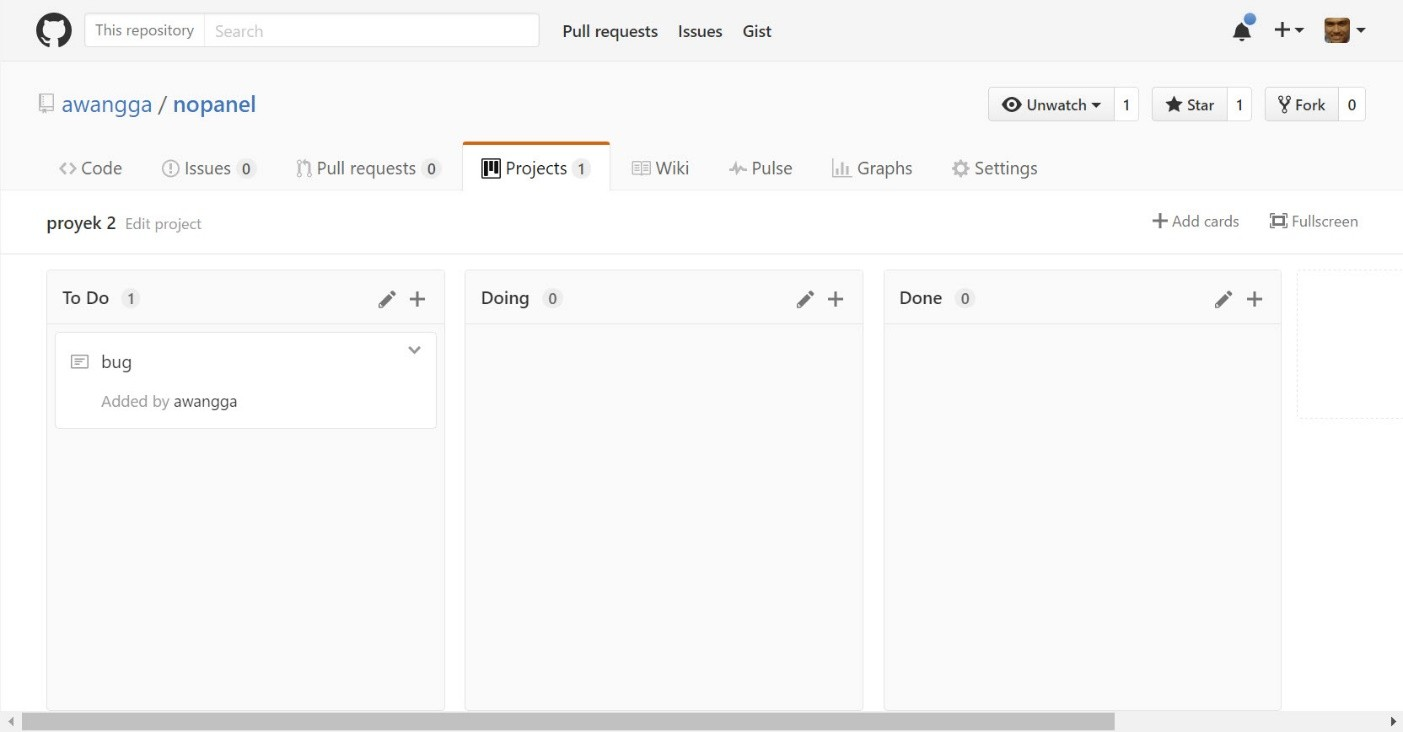
\includegraphics[scale=0.4]{figures/aad.jpg}
    \label{aasd}
\end{figure}

\textbf{\underline{Penting :}}\par
Git	ini	merupakan	alat	kontrol	pengembangan	aplikasi,	ingat!!!	dipakai	sejak	awal	mulai	mengkode	bukan	mengunggahnya	pada	saat	terakhir	sebelum	sidang	atau	anda	mendapat	nilai	0	
untuk	SCM(Source	Code	Management)/	Manajemen	Kode	Sumber.
\par 

Apabila	aplikasi	anda	tidak	dibuka	publik	atau	opensource	bisa	diganti	dengan	bitbucket	atau	
git.vas.web.id
\par 

Petunjuk	standar	github	dalam	bentuk	video	bisa	dibuka	melalui	link	berikut	:
\begin{enumerate}
\item Membuat	repositori	di	github	: \url{https://youtu.be/27JkHR59mmg}
\item Invite	User	: \url{https://youtu.be/gbxW8bQ29y0}
\item Menggunakan	git	scm	: \url{https://youtu.be/DpgfmeCZsCQ}
\end{enumerate}

\section{Petunjuk	Video	Standar}
Video	yang	dibuat	dibagi	menjadi	tiga	bagian	waktu	(linimasa)	dalam	satu	video, \textbf{waktu pembuka} yaitu	mulai	dari	menit	ke	nol,\textbf{waktu	penjelasan} disambung	setelah	waktu	pembuka,\textbf{waktu	penutup} disambung	setelah	waktu	penjelasan.
\\
\\
\textbf{Waktu Pembuka :}
\\
\begin{enumerate}
\item Video	muka	diri	sendiri	ukuran	setengah	badan	atau	lebih,	memperkenalkan	diri	dengan	nama,	kelas,	jurusan	dan	npm	beserta	nama	pembimbing	dan	jelaskan	keunggulan,	kelebihan	dan	kemampuan	anda (\textit{Nilai	20}).

\item . memberikan	latar	belakang	permasalahan	yang	akan	disolusikan	dengan	menggunakan	minimal	satu	alat	peraga	(minimal	papan	tulis	atau	alat	peraga	lainnya	yang	membantu	
penjelasan) (\textit{Nilai	20})
\end{enumerate}

\textbf{Waktu	Penjelasan	:}\\
video	penjelasan	wajib	terdiri	dari \textbf{teori	dan	praktek}.
\begin{enumerate}
\item Penjelasan	teori	menggunakan	alat	peraga, (\textit{Nilai	20})
\item kemudian	praktek	bisa	merekam	layar	laptop	untuk	praktek	pengkodean	atau	merekam	praktek	langsung	kondisi	di	lapangan. (\textit{Nilai	20})
\end{enumerate}

\textbf{Waktu	Penutup	:}
\begin{enumerate}
\item Berisi	kesimpulan	dan	saran (\textit{nilai 20})
\end{enumerate}

\section{Petunjuk	Standar	Tulisan	Blog}
Anda	bisa	menggunakan	blog	yang	digunakan	bersama	dalam	satu	kelompok	atau	kelas	jika	disepakati	seluruh	tulisan	dimasukkan	ke	satu	alamat	blog	saja	oleh	dosen,	atau	jika	diminta	di	blog	masing-masing	anda	bisa	menggunakan	Wordpress.com,	medium.com,kompasiana.com,	blogger.com. \\
Untuk	kepentingan	tugas	dan	bimbingan	dalam	bentuk	tulisan	di	blog,	memiliki	standar	baku	untuk	kerangka	penulisannya	harus	berisi	:\\
\textbf{Pembuka :}
\begin{enumerate}
\item Gambar	Ilustrasi	Buatan	Sendiri	Orisinil	(Nilai	20).
\item Latar	Belakang	Masalah	(nilai	20).
\end{enumerate}

\textbf{Isi :}
\begin{enumerate}
\item Tambahkan \underline{Video Standar} disini(Penilaian	Video	Terpisah).
\item Penjelasan	dan	solusi	masalah	(nilai	20).
\end{enumerate}

\textbf{Penutup :}
\begin{enumerate}
\item Kesimpulan	dan	saran	(nilai	20).

\item Tambahkan	URL \underline{Git	yang	sudah	Standar} disini(Penilaian	Git Terpisah).

\item Tambahkan	Nama,	NPM,	Kelas,	Prodi,	Kampus.

\item Link/URL	dengan	Nama	Matakuliah	diarahkan	ke	http://www.awangga.net/	atau	yg	disepakati	(Contoh	: \underline{Sistem	Informasi	Geografis}).

\item Referensi	atau	daftar	pustaka	(nilai	20).

\item Link/URL	menuju	skrinsut	Hasil	Scan \underline{ Plagiarisme}(Pilih	2	diantara	4	di	menu	Plagiarisme) yang	diupload	di	google	drive	(Wajib	ada,	jika	tidak	ada	atau	nilai	0)

\end{enumerate}

Penting	:	Sebelum	tulisan	anda	di	publish	di	blog,	untuk	di	scan	plagiarisme	terlebih	dahulu.	Seteleh	publish	scan	lagi	dengan	URL	blog	Plagiarisme	Checker.	Nilai	\%	plagiarisme	diambil	yang	paling	rendah	persentasenya. \\
Nilai	akhir	tulisan	=	Total	Nilai	Tulisan	(20+20+20+20+20)*Persentasi	(\%)	Uniqeness	hasil	scan	
plagiarisme.


\chapter{HAK DAN KEWAJIBAN PEMBIMBING, PENGUJI DAN MAHASISWA
DALAM PEKERJAAN PROYEK POLITEKNIK POS INDONESIA}

\section{Aturan	Baru}
Kesepakatan	program	Studi untuk	Bobot	Nilai	adalah	sebagai	berikut:

\begin{table}[H]
\label{anjay}
\begin{tabular}{lll}
Pembimbing &  & : 65\% \\
Penguji &  & : 35\%
\end{tabular}
\end{table}

\section{Hak	dan	Kewajiban	Pembimbing}
\begin{enumerate}
\item Pembimbing	 berhak	 sepenuhnya	 menyetujui	 atau	 menolak	 mahasiswa	 bimbingannya	untuk	mengikuti	siding .
\item Pembimbing	harus	mendampingi	mahasiswa	selama	sidang	berlangsung .
\item Pembimbing	 diharuskan	 memberikan	 nilai	 Evaluasi	 Pelaksanaan Proyek	 sebelum	mahasiswa	bimbingannya	siding .
\item Pembimbing	 tidak	 diperkenankan	 menjawab	 pertanyaan	 Penguji	 untuk	 Mahasiswa,	kecuali	diminta	oleh	Penguji .
\item Pembimbing	berpakaian	rapi	dan	berdasi	selama	sidang.
\end{enumerate}

\section{Hak	dan	Kewajiban	Penguji}
\begin{enumerate}
\item Penguji	harus	sudah	datang	15	menit	sebelum	sidang	Proyek	dimulai.
\item Penguji	yang	terlambat	lebih	dari	15	menit	dari	waktu	sidang	yang	telah	ditetapkan	akan	
digantikan	oleh	Penguji	Pengganti.
\item Bila	tidak	ada	alasan	yang	kuat	atas	ketidak	hadiran	Penguji,	maka	Surat	Tugas	dan	Honor	
akan	dialihkan	kepada	Penguji	Pengganti.
\item Tim	Penguji	berhak	membatalkan	sidang	jika	Mahasiswa	terlambat	atau	tidak	hadir	sesuai	
jadwal	yang	telah	ditetapkan.
\item Tim	 penguji	 berhak	 membatalkan	 sidang,	 apabila	 pernyataan	 pembimbing	 tidak	 benar	(Tulisan	selesai	100\%	dan	Materi	Proyek	$\geq90\%$).
\item Sidang	akan	tetap	berlangsung	bila	2	(dua)	Penguji	(Ketua	Penguji	dan	Anggota	Penguji)	
hadir.
\item Berdasarkan	 proses	 sidang,	 Tim	 Penguji	 berhak	 sepenuhnya	 menetapkan	 status	 akhir	
sidang	tersebut,	yaitu	LULUS/LULUS	BERSYARAT/TIDAK	LULUS.
\item Ketua	 Penguji	 	 dan	 Anggota	 Penguji	 harus	 memberikan	 nilainya	 diakhir	 sidang	 secara	
objektif	dengan	tidak	melihat	Nilai	yang	diberikan	oleh	Penguji/Pembimbing	lain.
\item Ketua	 Penguji	 harus	 menghitung	 diakhir	 sidang	 Nilai	 Akhir	 yang	 dikumpulkan	 secara	
serentak	dari	Seluruh	Penguji	dan	Pembimbing	dengan	menggunakan	aturan/rumus	yang	
telah	ditetapkan.
\item Ketua	 Penguji	 harus	 mengkoordinasikan	 perbedaan	 nilai	 antar	 Penguji	 melalui	 proses	
debat/forum	diskusi	agar	didapat	nilai	yang	objektif	(Setiap	nilai	harus	berada	pada	range	
yang	sama,	misal	A,	B,	atau	C).
\item Ketua	Penguji	harus	mengumumkan	Nilai	Akhir	kepada	Mahasiswa	selesai	siding.
\item Penguji	berpakaian	rapi	dan	berdasi.
\end{enumerate}

\section{Hak	Dan	Kewajiban	Mahasiswa	Peserta	Sidang}
\begin{enumerate}
\item Mengikuti	jadwal	sidang	Proyek	oleh	Panitia.
\item Menyerahkan	 Surat	 Persetujuan	 Sidang	 dari	 Pembimbing	 sesuai	 waktu	 yang	 telah	
ditetapkan	oleh	Panitia.
\item Menyerahkan	 draf	 Laporan	 Proyek	 yang	 akan	 disidangkan	 kepada	 para	 penguji	 paling	
lambat	1	(satu)	hari	sebelum	sidang	dilaksanakan.
\item Hadir	30	menit	sebelum	sidang	dimulai.
\item Mempersiapkan	peralatan	sidang	yang	dibutuhkan.
\item Memakai	pakaian	seragam	dan	jas	almamater.
\item Berhak	mendapatkan	hasil	Evaluasi	Sidang	dari	tim	Penguji.
\end{enumerate}

\section{Prosedur Pelaksanaan	Sidang	Proyek	}
\begin{enumerate}
\item Waktu	pelaksanaan	sidang	1,5	jam	untuk	setiap	judul.
\item Sidang	dipimpin	oleh	Ketua	Penguji	(Pembimbing).
\item Pelaksanaan	sidang	sebagai	berikut :
	\begin{enumerate} [label=(\alph*)]
		\item Pembukaan	oleh	Ketua	Penguji. 
		\item Presentasi	Proyek	oleh	Mahasiswa		(maks.	15	menit).
		\item Demonstrasi	alat	dan	Tanya-jawab	(maks.	60	menit).
		\item Rapat	tertutup	penentuan	dan	diskusi	nilai	Tim	Penguji	(maks.	15	menit).
	\end{enumerate}
\end{enumerate}

\begin{figure}[H]
    \centering
    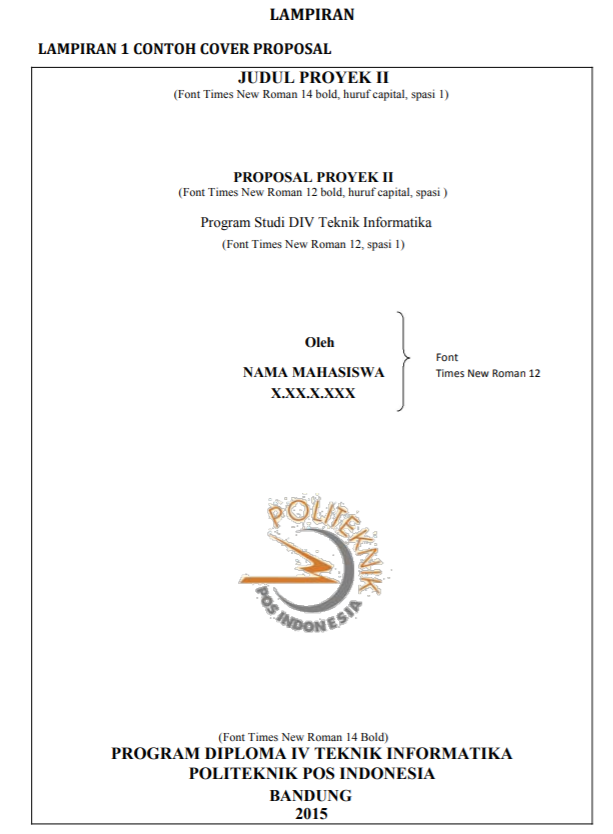
\includegraphics[scale=0.9]{figures/lap1.png}
    \label{alir}
\end{figure}

\begin{figure}[H]
    \centering
    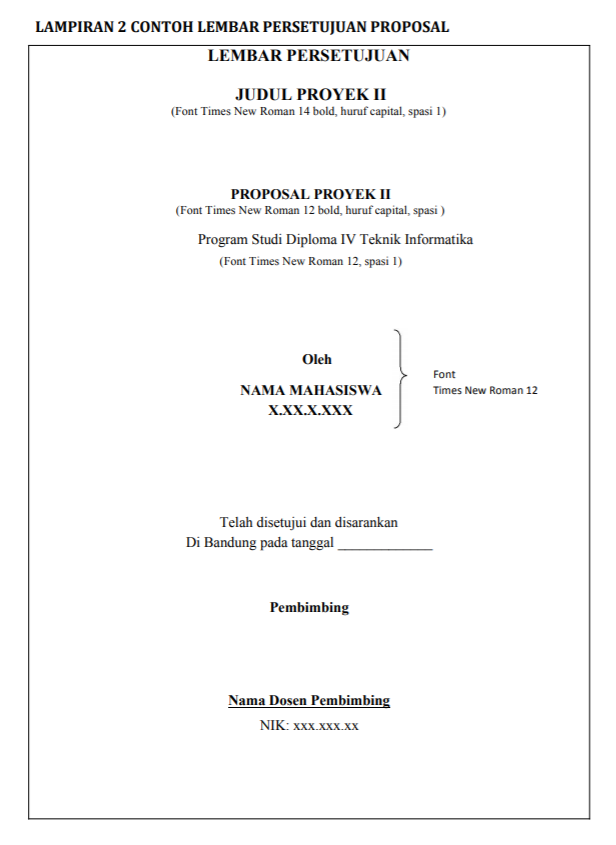
\includegraphics[scale=0.9]{figures/lap2.png}
    \label{alir}
\end{figure}



%now enable appendix numbering format and include any appendices
%\appendix
%\chapter{Form Penilaian Jurnal}

gambar \ref{form1} dan \ref{form2} merupakan contoh bagaimana reviewer menilai jurnal kita. 
\begin{figure}[ht]
      \centerline{\includegraphics[width=1\textwidth]
      {figures/form1}}
      \caption{Form nilai bagian 1.}
      \label{form1}
      \end{figure}

	\begin{figure}[ht]
	      \centerline{\includegraphics[width=1\textwidth]
	      {figures/form2}}
	      \caption{form nilai bagian 2.}
	      \label{form2}
	      \end{figure}

%\chapter{FAQ}

M : Kalo Intership II atau TA harus buat aplikasi ?
D : Ga harus buat aplikasi tapi harus ngoding

M : Pa saya bingung mau ngapain, saya juga bingung mau presentasi apa?
D : Makanya baca de, buka jurnal topik `ganteng' nah kamu baca dulu sehari 5 kali ya, 4 hari udah 20 tuh. Bingung itu tanda kurang wawasan alias kurang baca.

M : Pa saya sudah cari jurnal terindeks scopus tapi ga nemu.
D : Kamu punya mata de? coba dicolok dulu. Kamu udah lakuin apa aja? tolong di list laporkan ke grup Tingkat Akhir. Tinggal buka google scholar klik dari tahun 2014, cek nama jurnalnya di scimagojr.com beres.

M : Pa saya belum dapat tempat intership, jadi ga tau mau presentasi apa?
D : kamu kok ga nyambung, yang dipresentasikan itu yang kamu baca bukan yang akan kamu lakukan.

M : Pa ini jurnal harus yang terindex scopus ga bisa yang lain ?
D : Index scopus menandakan artikel tersebut dalam standar semantik yang mudah dipahami dan dibaca serta bukan artikel asal jadi. Jika diluar scopus biasanya lebih sukar untuk dibaca dan dipahami karena tidak adanya proses review yang baik dan benar terhadap artikel.

M : Pa saya tidak mengerti
D : Coba lihat standar alasan

M : Pa saya bingung
D : Coba lihat standar alasan

M : Pa saya sibuk
D : Mbahmu....

M : Pa saya ganteng
D : Ndasmu....

M : Pa saya kece
D : wes karepmu lah....


Biasanya anda memiliki alasan tertentu jika menghadapi kendala saat proses bimbingan, disini saya akan melakukan standar alasan agar persepsi yang diterima sama dan tidak salah kaprah. Penggunaan kata alasan tersebut antara lain :

1. Tidak Mengerti : anda boleh menggunakan alasan ini jika anda sudah melakukan tahapan membaca dan meresumekan 15 jurnal. Sudah mencoba dan mempraktekkan teorinya dengan mencari di youtube dan google minimal 6 jam sehari selama 3 hari berturut-turut.

2. Bingung : anda boleh mengatakan alasan bingung setelah maksimal dalam berusaha menyelesaikan tugas bimbingan dari dosen(sudah dilakukan semua). Anda belum bisa mengatakan alasan bingung jika anda masih belum menyelesaikan tugas bimbingan dan poin nomor 1 diatas. Setelah anda menyelesaikan tugas bimbingan secara maksimal dan tahap 1 poin diatas, tapi anda masih tetap bingung maka anda boleh memakai alasan ini.

%next line adds the Bibliography to the contents page
\addcontentsline{toc}{chapter}{Daftar Pustaka}
%uncomment next line to change bibliography name to references
%\renewcommand{\bibname}{References}
\bibliography{references}        %use a bibtex bibliography file refs.bib
\bibliographystyle{plain}  %use the plain bibliography style

\end{document}

